\documentclass[12pt]{article}
\usepackage{setspace} 
\usepackage{geometry}
\usepackage{enumitem}
\usepackage{lipsum}
\usepackage{hyperref}
\usepackage{lineno}
\usepackage{makecell}
\usepackage[T1]{fontenc}

%\usepackage[utf8]{inputenc}
\usepackage{natbib}

% final or draft
\usepackage[draft]{changes}

\usepackage{cite}
\usepackage[ruled]{algorithm2e}
\usepackage{amsmath,amssymb,amsfonts}
\usepackage{graphicx}
\usepackage{textcomp}
\usepackage{multirow}
\usepackage{subcaption}
\usepackage{xcolor}
\usepackage{indentfirst}
\def\BibTeX{{\rm B\kern-.05em{\sc i\kern-.025em b}\kern-.08em
    T\kern-.1667em\lower.7ex\hbox{E}\kern-.125emX}}

\geometry{margin=1in}

% Enable line numbering
\linenumbers

% footnote email
\newcommand\blfootnote[1]{
    \begingroup
    \renewcommand\thefootnote{}\footnote{#1}
    \addtocounter{footnote}{-1}
    \endgroup
}

% reset space of equation blocks
\usepackage{etoolbox}
\AtBeginEnvironment{equation}{\setstretch{1}\vspace{-0\baselineskip}}
\AtBeginEnvironment{align}{\setstretch{1}\vspace{-\baselineskip}}
% remove double space for references
\AtBeginEnvironment{thebibliography}{\linespread{1}\selectfont}

\begin{document}

% Title
% \title{GrapeCPNet: A deep learning integration for grape completion and phenotyping in 3D}
\title{\added{GrapeCPNet: A Self-supervised Point Cloud Completion Network for 3D Phenotyping of Grape Bunches}}
\author{
    Wenli Zhang \textsuperscript{a,*},
    Chao Zheng \textsuperscript{a},
    Chenhuizi Wang \textsuperscript{a},
    Pieter M. Blok \textsuperscript{b}, \\
    Haozhou Wang \textsuperscript{b},
    Wei Guo \textsuperscript{b,*}
    \blfootnote{Corresponding author: zhangwenli@bjut.edu.cn; guowei@g.ecc.u-tokyo.ac.jp }
    \blfootnote{Email addresses: zhengchao97201@163.com (Chao Zheng), Wangchenhuizi@emails.bjut.edu.cn (Chenhuizi Wang), pieter.blok@fieldphenomics.com (Pieter M. Blok), haozhou-wang@g.ecc.u-tokyo.ac.jp (Haozhou Wang), guowei@g.ecc.u-tokyo.ac.jp (Wei Guo)}
}
\date{}

\maketitle

% Footnotes for authors
\noindent\textsuperscript{a} Information Department, Beijing University of Technology, Beijing, China \\
% Email: zhangwenli@bjut.edu.cn \\
\textsuperscript{b} Graduate School of Agricultural and Life Sciences, The University of Tokyo, Tokyo, Japan\\
% \textsuperscript{*} \\

\textbf{\added{Highlights}}


\begin{itemize}
%   \item Novel deep learning pipeline for automated 3D grape phenotyping.
%   \item GrapeCPNet: Self-supervised network for berry points cloud completion.
%   \item High accuracy in berry instance segmentation (99.5\% average precision).
%   \item Robust performance across four grape varieties ($R^2$ of 0.855 for radius, 0.969 for 
% volume).
%   \item Non-destructive and high-throughput analysis for viticulture applications.
  \item \added{GrapeCPNet completes 3D point clouds for segmented berry instances.}
  \item \added{GrapeCPNet is trained using self-supervision, free of manual annotations.}
  \item \added{Integrated into a deep learning pipeline for automated 3D grape bunch phenotyping.}
  \item \added{Achieved over 0.85 $R^2$ and 99.5\% average precision on four grape varieties.}
\end{itemize}

\begin{abstract}
The measurement of phenotypic parameters of fresh grapes, especially at the individual berry level, is critical for yield estimation and quality control. 
Currently, these measurements are done by humans, making it costly, labor-intensive, and often inaccurate. 
Advances in 3D reconstruction and point cloud analysis allow extraction of detailed traits for grapes, yet current methods struggle incomplete point clouds due to occlusion. 
This study presents a novel deep-learning-based phenotyping pipeline designed specifically for 3D point cloud data.                                                         
First, individual berries are segmented from the grape bunch using the SoftGroup deep learning network. 
Next, a self-supervised point cloud completion network, termed GrapeCPNet, addresses occlusions by completing missing areas.  
Finally, morphological analyses are applied to extract berry radius and volumes. 
Validation on a dataset of four fresh grape varieties yielded  $R^2$ values of 85.5\% for berry radius and 96.9\% for berry volume, respectively. 
These results demonstrate the potential of the proposed method for rapid and practical extraction of 3D phenotypic traits in grape cultivation.
\end{abstract}

\textbf{Keywords:} 3D point cloud analysis, instance segmentation, shape completion

\doublespacing

\section{Introduction}
Fresh grape is one of the most important agricultural products and economic crops \citep{alston_grapes_2019}. 
Its global production and consumption is increasing year by year. 
To \replaced{effectively}{better} guide planting strategies and monitoring growing status, several geometric parameters\replaced{, including}{like counts, length, and volume at bunch level and berry level are commonly used in actual applications raihen\_prediction\_2024.} 
\deleted{Among them,} the number \deleted{and the radius }of \deleted{the} berries \replaced{and their radius, are frequently measured}{are the most important phenotypic parameters (sneha\_acrescale\_2024) }. 
Traditional manual \replaced{measuring}{phenotyping of }traits is labor-intensive and time-consuming, and often destructive. 
To reduce the cost and increase the efficiency, the non-destructive and high-throughput acquisition of phenotypic traits based on computer vision has attracted extensive interest in recent years. 
Several simple geometry traits can be acquired from 2D images by using computer vision algorithms that use pattern recognition, machine learning, and deep learning \citep{chen_instance_2023, zabawa_counting_2020}. 
Projecting the 2D image plane onto the 3D world inevitably results in information loss. 
The occlusion of berries often lead to incomplete representations of grape bunches. 
Additionally, clustered berries and their shadows create challenges for obtaining reliable measurements of phenotypic parameters through 2D image analysis, even under controlled lightning conditions.

Advances in 3D scanning and reconstruction techniques have made it possible to retain detailed spatial information about objects, enabling the acquisition of complex 3D morphological traits in grape bunches \citep{ni_threedimensional_2021}. 
Researchers have developed 3D phenotyping processes for grapes by combining feature-engineered point cloud processing algorithms \citep{rose_automated_2016, rist_highprecision_2018}. 
These methods primarily rely on point cloud segmentation techniques, such as edge-based segmentation, region-growing segmentation, and sphere-fitting algorithms. 
Unfortunately, traditional point cloud processing algorithms heavily rely on prior knowledge of the target object and require extensive manual feature engineering and parameter tuning to achieve optimal results in a wide range of conditions, thereby limiting their generalization performance.
\added{Implementing} state-of-the-art deep learning approaches\replaced{, which automatically learn features}{use a data-driven feature learning} from the point cloud data \replaced{, can  reduce the workload of designing robust algorithms for complex and diverse conditions}{ automatically}.
\deleted{It recently shows promising adaptability and accuracy in plant 3D phenotyping (schneider\_predicting\_2020, scholer\_automated\_2015). }
\deleted{Focusing on point cloud segmentation applications, }
\deleted{li\_maspc\_2022 proposed MASPC\_Transform to segment the stems and leaves of rose bush point cloud data to obtain 3D phenotypic parameters. }
\deleted{wang\_3d\_2022 realized leaf instance segmentation by designing the PartNet for lettuce point cloud data. }
\deleted{li\_psegnet\_2022 proposed PSegNet for segmenting stems and leaves of tomato, tobacco, and sorghum. }
\replaced{However, few studies have reported good performance deep learning networks and pipelines in}{The previous studies focused on canopy level or individual plant level analysis, and demonstrated that instance segmentation alone is insufficient on} berry level analysis. 

\added{Another challenge after the success of instance berry segmentation is the incomplete representation of berry surfaces.} 
The aggregated cluster growth causes the berries to squeezed against each other, leading to self occlusion and resulting in an incomplete point cloud of berry surfaces \citep{du_instance_2023}. 
Therefore, point cloud instance segmentation can only capture partial information rather than that of whole berries.
To address \replaced{this issue}{the issue of partial point clouds,} and consequently an underestimation of the berry traits, point cloud shape completion is one of the most commonly used solutions.
Point cloud completion is the task of generating a complete 3D shape given partial point cloud input \citep{tesema_point_2024}. 
For instance, \citet{ge_symmetrybased_2020} assume that strawberries are symmetrical, suggesting that their shape can be completed by mirroring the existing shape, provided an appropriate symmetrical plane can be identified.
\citet{marangoz_fruit_2022} proposed an super-ellipsoids matching approach to map fruits on plants and estimate their shape.
However, these methods are limited to specific fruit characteristics and require manual design of algorithms according to the features of the fruit, lacking the potential for generalized application.
Utilizing deep learning methods, researchers have designed point cloud completion networks \citep{wang_unsupervised_2021}. 
\citet{park_deepsdf_2019} introduced DeepSDF to achieve the completion of object point cloud models. It uses a learned continuous signed distance function to represent a class of shapes in latent space and is tolerant to noisy 3D input data. 
\citet{magistri_contrastive_2022} utilized DeepSDF and its latent space in an encoder-decoder network that converted a single RGB-D frame to a 3D shape of a complete fruit. 
This encoder-decoder network was extended and optimized by \citet{blok_highthroughput_2025} for high-throughput 3D shape completion of potato tubers on a commercial harvester. 
\deleted{Outside the agricultural domain, tang\_lakenet\_2022 proposed a point cloud completion network (Lake-net) for furniture model point cloud datasets.} 
For grape berry application, the shape of the berry can be roughly approached by the deformation of a sphere or ellipsoid depending on the species. 
Existing datasets from other fruits cannot be applied directly, and manually creating paired training datasets is time-consuming and labor-intensive.
Therefore, there is a demand to develop an analysis pipeline, capable of completing the detailed surface of an incomplete berry point cloud while requiring less labor-intensive training data preparation.

In this study, we proposed a novel berry-level 3D grape phenotyping pipeline that will overcome the occlusion issues. 
The proposed pipeline includes: 
(1) a individual berry segmentation module that segment each berry from 3D point cloud of whole bunch; 
(2) a point cloud completion module that complete the missing part of segmented berry point cloud data through automatic training data generation; 
(3) a phenotyping module that extract berry phenotypic traits including radius and volume. 
\replaced{The proposed pipeline was evaluated}{The novelty of our study is the research of this novel pipeline and its evaluation} on four different fresh grape species (Red, Green, Kyoho, and Shine Muscat Grape).

\section{Materials and Methods}

In this section, we first introduce the plant material for our grape analysis, followed by the 3D reconstruction methods for obtaining 3D point cloud data. 
We then provide a brief overview of the SoftGroup \citep{vu_softgroup_2022} deep learning network, which was trained on our point cloud dataset for instance segmentation of individual berries (Fig.~\ref{fig:raw1}a). 
Next, we detail the proposed self-supervised completion deep learning module, GrapeCPNet, which predicts the complete berry point cloud from segmented partial berries (Fig.~\ref{fig:raw1}b). 
Subsequently, we describe the module and method for calculating phenotypic traits (Fig.~\ref{fig:raw1}c). 
Finally, we introduced the evaluation method for model training and results validation.

% fig.1
\begin{figure}[hbt!]
    \centering
    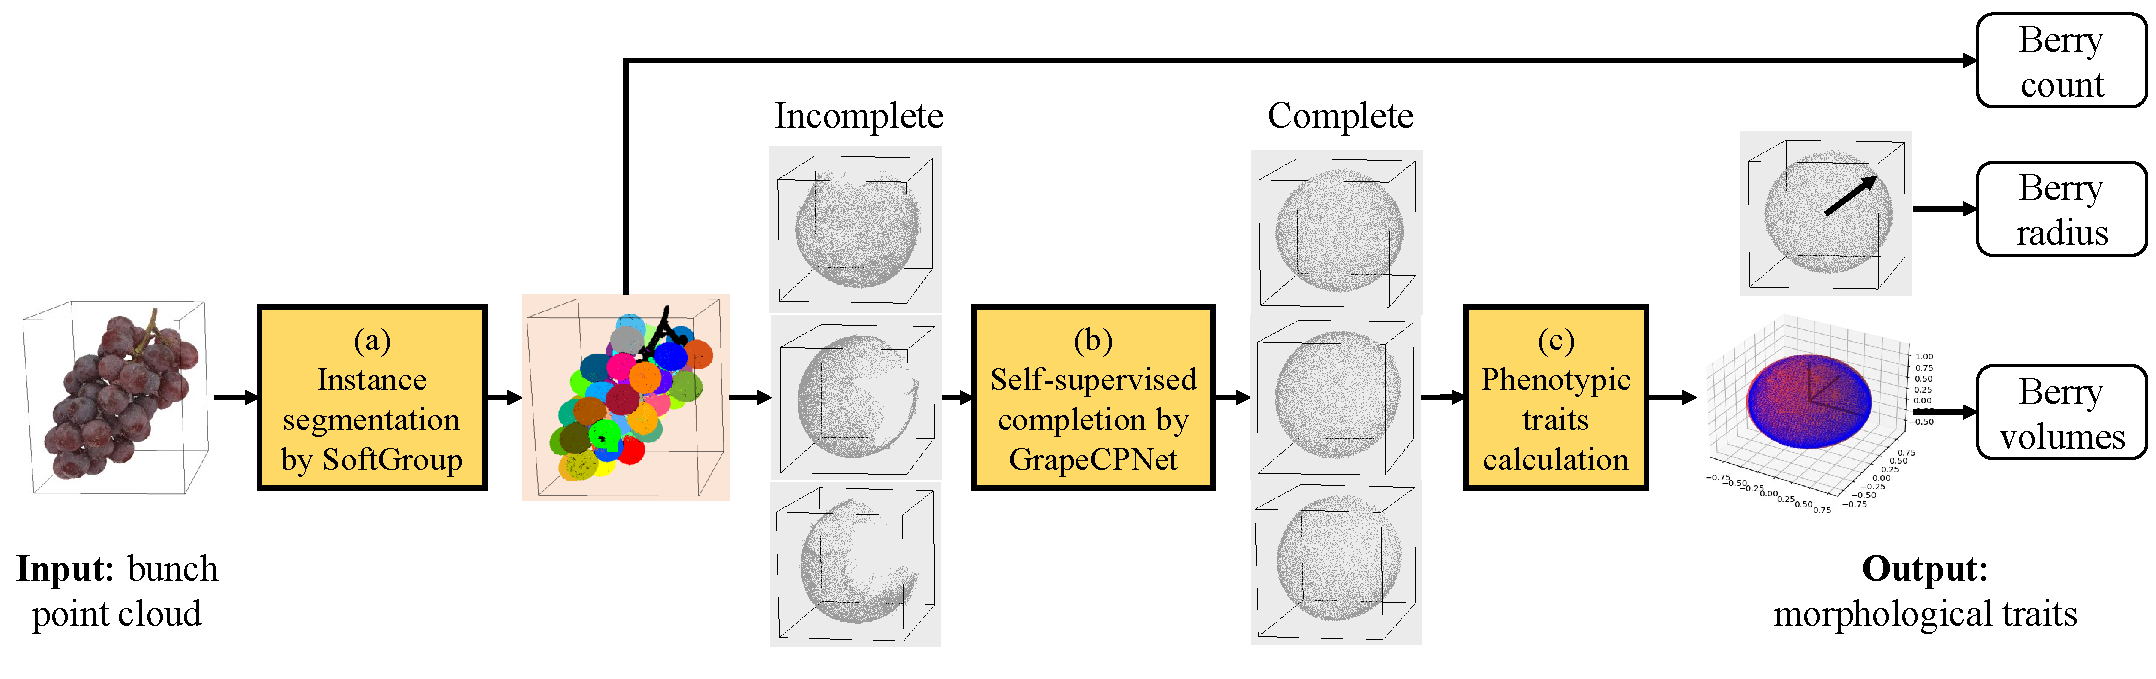
\includegraphics[width=1\textwidth]{figures/Figure1.pdf}
    \caption{Proposed pipeline for grape bunch 3D phenotyping. Taking the bunch point cloud data as input, it is realized through three steps: (1) berry instance segmentation by SoftGroup \citep{vu_softgroup_2022}, (2) berry point cloud completion by proposed GrapeCPNet, and (3) phenotypic traits calculation.}
    \label{fig:raw1}
\end{figure}

\subsection{Plant Materials and Point Cloud Acquisition}

\subsubsection{Grape species}

To ensure the generalization and broad application of our study, this paper considers the sparsity, shape, and color of the bunch, and chooses four common fresh grapes as the experimental materials, which are Red Grape, Green Grape, Kyoho Grape, and Shine-Muscat Grape. 
The characteristics of them are shown in Table~\ref{tbl:1} and the examples are shown in Figure~\ref{fig:raw86}.

% table 1
\begin{table}[h]
    \centering
    \caption{Comparison of the characteristics of the four species of fresh grape}
    \begin{tabular}{cccc}
        \hline
        \textbf{Grape Species} & \textbf{Color} & \textbf{Sparsity} & \textbf{Shape} \\
        \hline
        Red & Purple-red & Sparser & Ellipsoid \\
        Green & Green & Sparse & Ellipsoid \\
        Kyoho & Dark-purple & Dense & Sphere \\
        Shine-Muscat & Green & Very dense & Sphere \\
        \hline
    \label{tbl:1}
    \end{tabular}
\end{table}

% fig.8 + fig.6 -> Fig.2
\begin{figure}[hbt!]
    \centering
    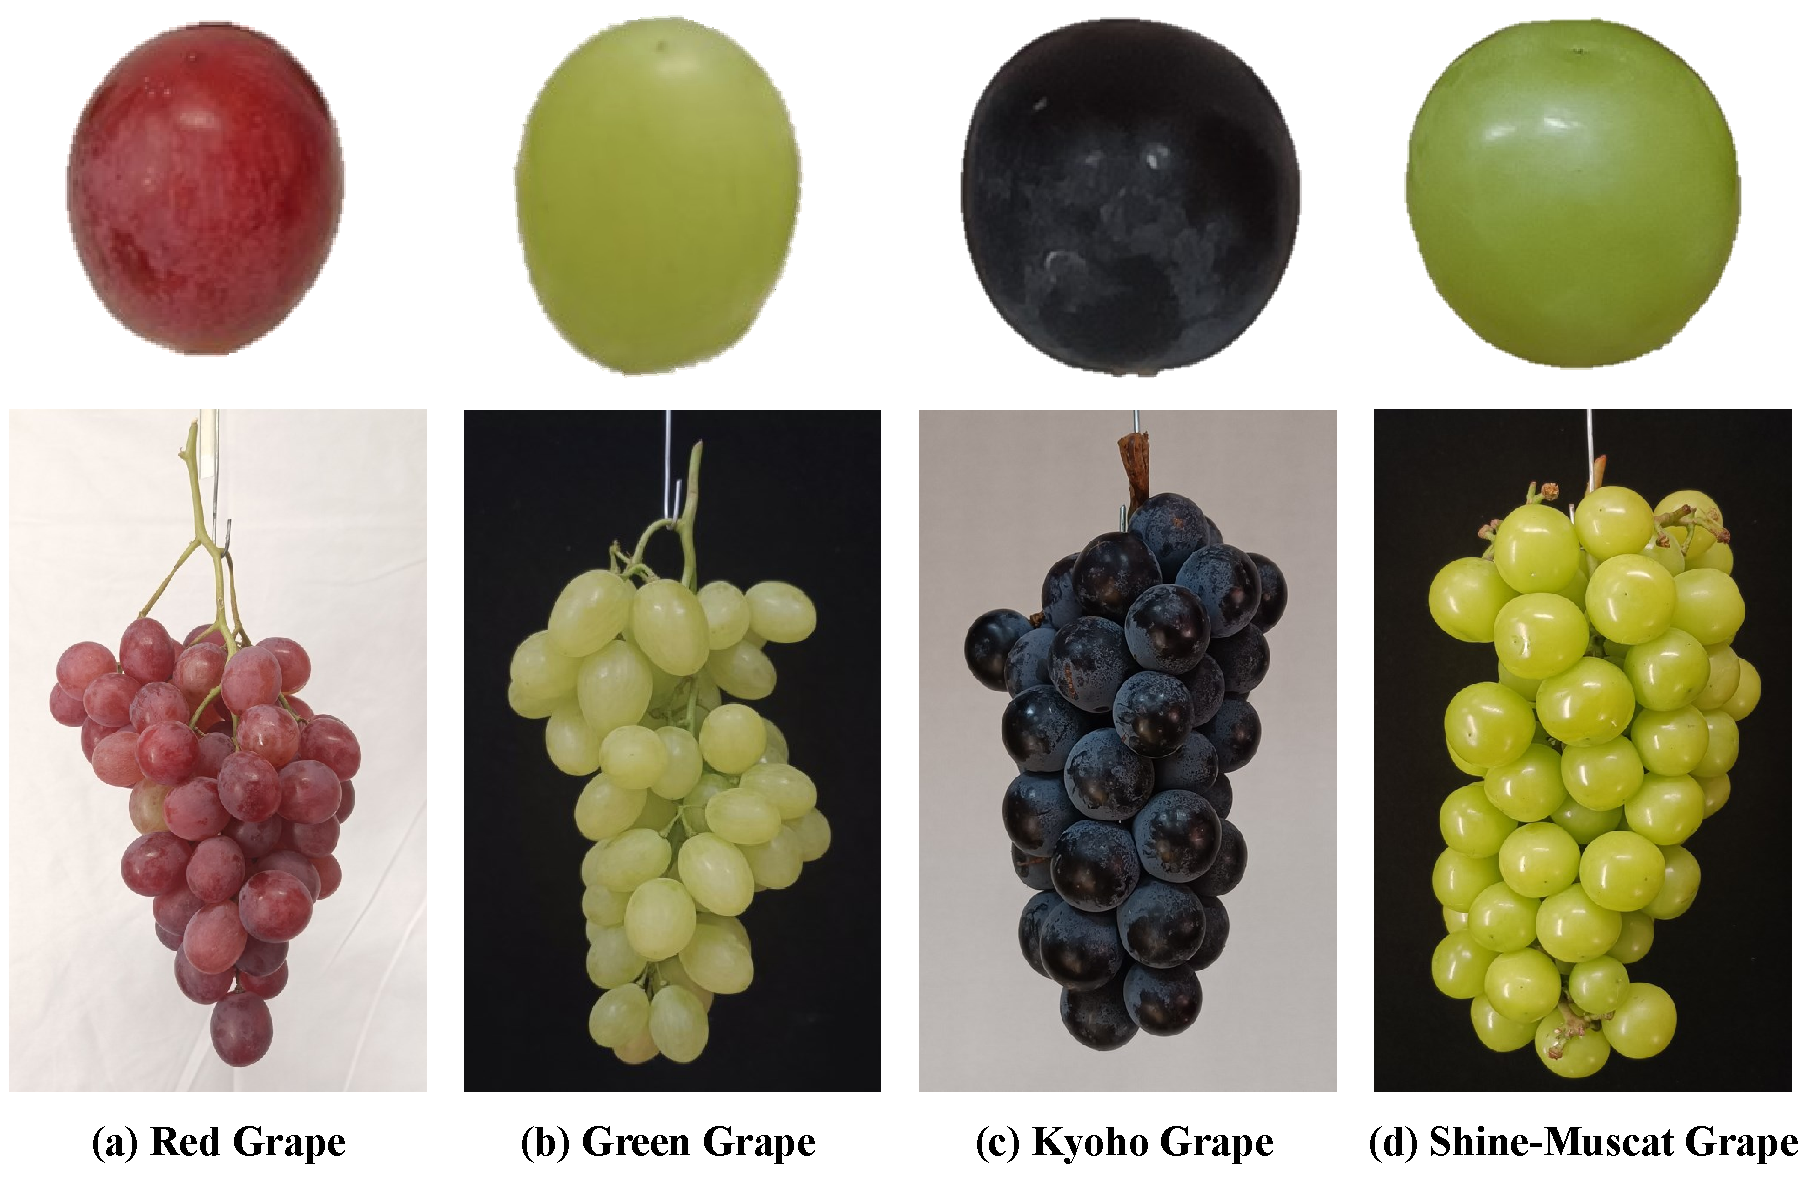
\includegraphics[width=1\textwidth]{figures/Figure2.pdf}
    \caption{Examples of four fresh grape bunches and their berries}
    \label{fig:raw86}
\end{figure}

\subsubsection{3D reconstruction of grape}
\label{sec:212}

In this paper, the multi-view images acquisition and 3D reconstruction by Agisoft Metashape (Agisoft LLC, St. Petersburg, Russia) was used to obtain the 3D point cloud of bunch (Fig.~\ref{fig:raw9}a) and single complete berry (Fig.~\ref{fig:raw9}b). 
Their correspondence of the same berry was also labeled as shown in Figure~\ref{fig:raw9}c.

% fig.9
\begin{figure}[hbt!]
    \centering
    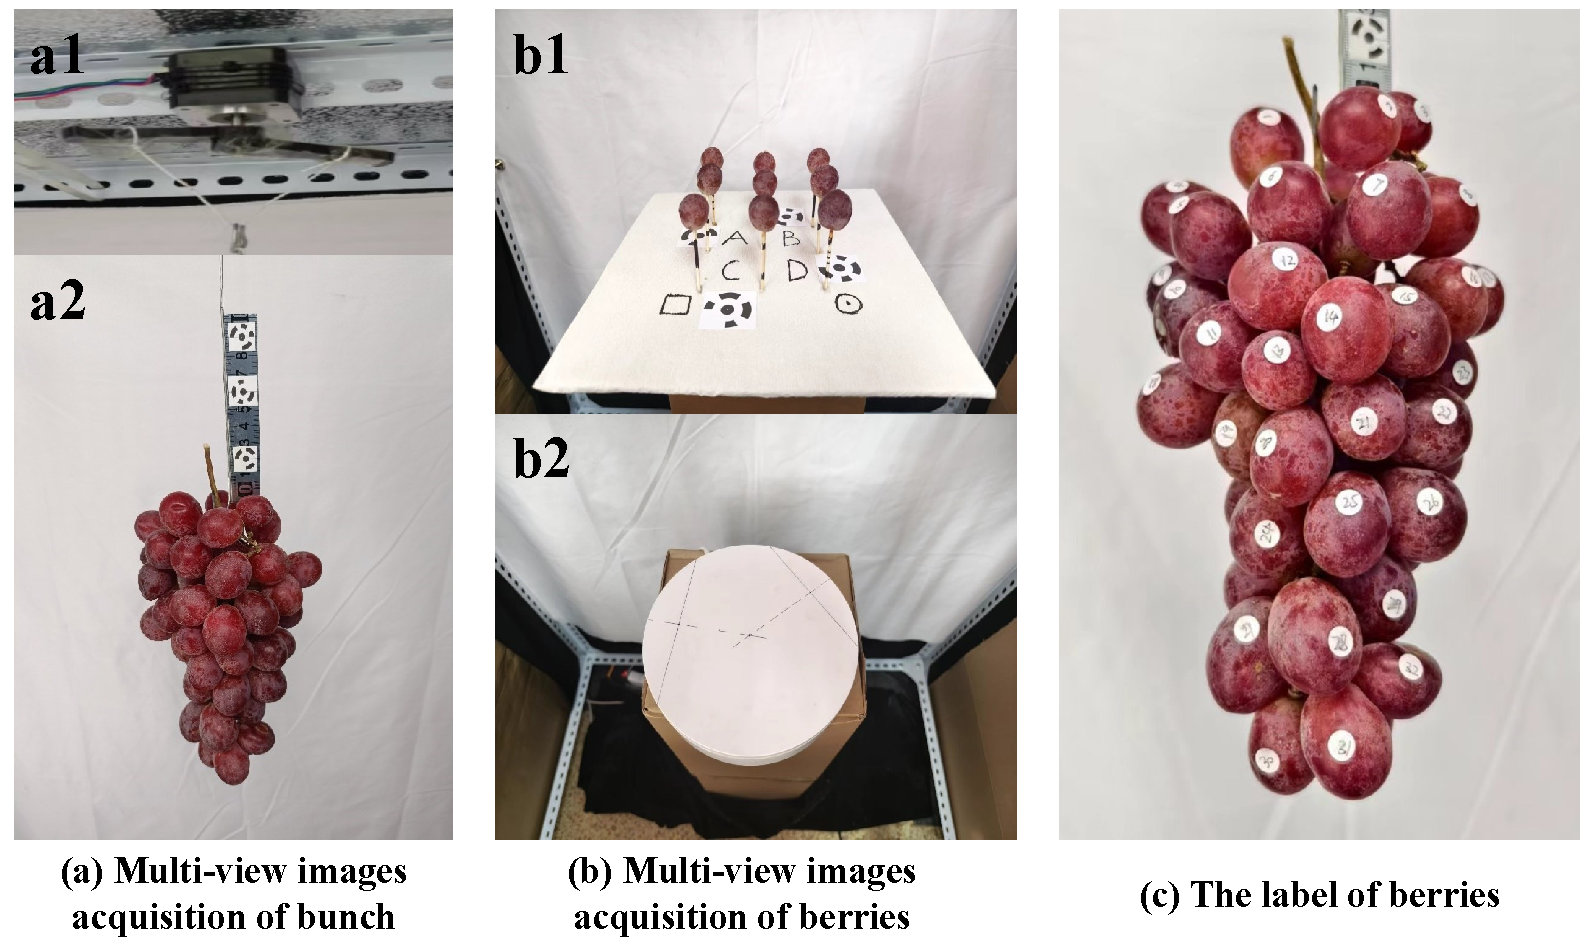
\includegraphics[width=1\textwidth]{figures/Figure3.pdf}
    \caption{Methods for obtaining multi-view images of bunch reconstruction and berry reconstruction, and the example of berry labeling}
    \label{fig:raw9}
\end{figure}

For whole bunch multi-view images acquisition, the device was built as shown in Fig.~\ref{fig:raw9}a. 
One grape bunch was hung on the hook which was attached to propellers driven by stepping motors (Fig.~\ref{fig:raw9}a1) that can achieve rotation at a certain speed. 
The entire device was placed in front of a solid-colored backdrop (Fig.~\ref{fig:raw9}a2), and multiple cameras were set up to photograph the bunch from different heights and view angles. 
In addition, a ruler with markers were used for scale correction. 
For single complete berry multi-view images acquisition in batch (Fig.~\ref{fig:raw9}b), 
nine berries were fixed floating by needle disk (Fig.~\ref{fig:raw9}b1) on a turntable (Fig.~\ref{fig:raw9}b2). 
The background, cameras, and marker settings are similar to the previous bunch reconstruction. 
The number of reconstructed images and the image acquisition parameters are selected, as shown in Table~\ref{tbl:2}. 
Examples of the point cloud of bunch, multiple berries, and single complete berries from multiple berries are shown in Figure~\ref{fig:raw10}.

% table 2
\begin{table}[h]
    \centering
    \caption{Image acquisition details for grape bunches and single berries}
    \begin{tabular}{ccccc}
        \hline
        \textbf{Object} & \textbf{Distance} & \textbf{Camera view angles} & \textbf{Rotation angles} &  \textbf{Total image \#} \\
        \hline
        Bunch        & 25-60cm & $0^{\circ}$, $\pm 25^{\circ}$, $\pm 45^{\circ}$ & $7.2^{\circ}$ (50 images) & $250$ \\
        Single berry & 20-40cm & $-15^{\circ}$, $0^{\circ}$, $25^{\circ}$, $45^{\circ}$ & $7.2^{\circ}$ (50 images) & $200$ \\
        \hline
    \label{tbl:2}
    \end{tabular}
\end{table}

% figure 10
\begin{figure}[hbt!]
    \centering
    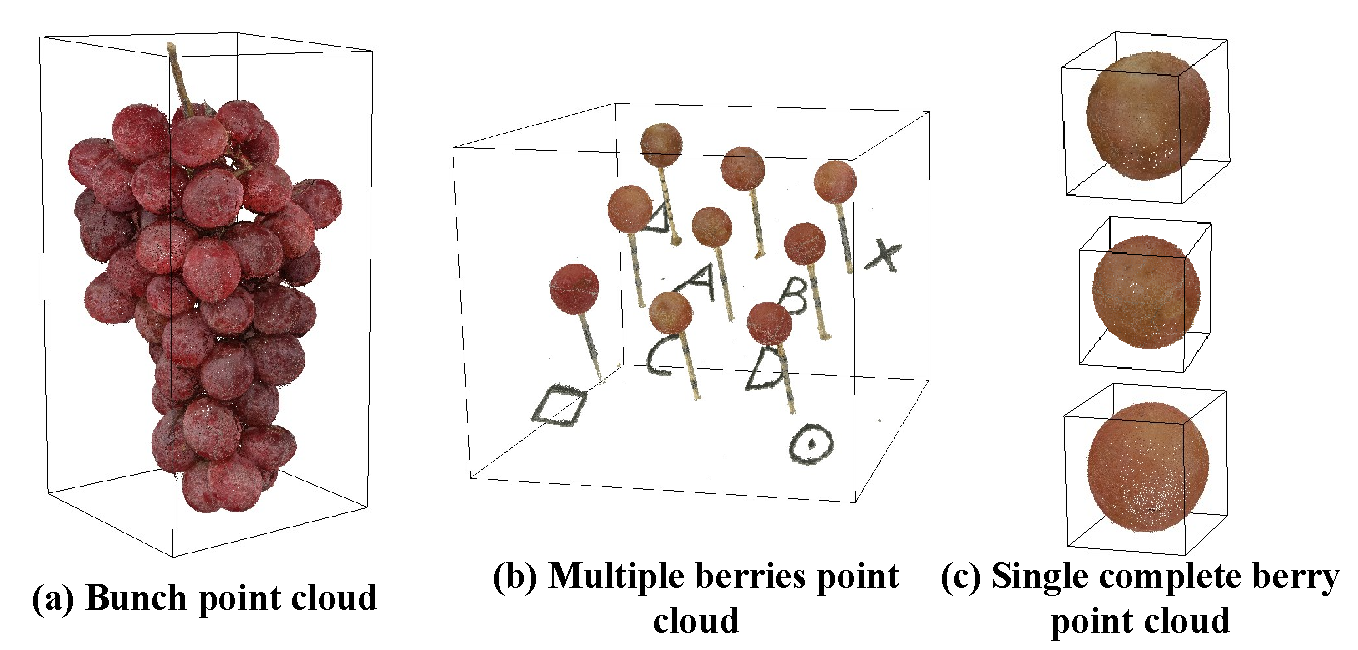
\includegraphics[width=1\textwidth]{figures/Figure4.pdf}
    \caption{Example of point cloud obtained based on multi-view images reconstruction}
    \label{fig:raw10}
\end{figure}

\subsection{Berry Instance Segmentation}
\label{sec:22}

As Figure~\ref{fig:raw1}a, the single-bunch shell point cloud was represented as $P_{bunch}=\{p_i \mid i=1, \cdots, m\}$, where $p_i=(x_i,y_i,z_i)$ denotes a point in 3D space and $m$ denotes the total number of points in the point cloud of the bunch. The bunch point cloud segmentation task expects to segment $P_{bunch}$ into a combination of several individual subsets of the berries point cloud and a subset of the stem point cloud, as shown in Equation~(\ref{eq:1}).

\begin{equation}
P_{bunch} = \sum_{i=1}^{n} P_{berry_{i}} + P_{stem}
\label{eq:1}
\end{equation}

{\raggedright where, $P_{berry_{i}}$ denotes the subset point cloud of the $i^{\text{th}}$ berry in the bunch, $n$ denotes the number of all the berries contained in the bunch, and $P_{stem}$ denotes the set of stem point cloud. 
Meanwhile, each subset $P_{berry_{i}}=\{p_i \mid i=1, \cdots, k\}$ consists of multiple points in 3D space, which can represent the location and morphology of the visible part of the berry within the bunch.}

The task of instance berry segmentation from a bunch is complex. 
As shown in Figure~\ref{fig:raw2}, it involves distinct localization features and complex boundary morphology. 
The distinct localization feature implies that individual berry has more geometrical and morphological details compared to the overall shape of the grape bunch, particularly when the object is a small-sized point cloud \citep{luo_infield_2022}. 
The complex boundary morphology arises from berries pressing against each other, resulting in multiple curves with varying connecting depths. 
Therefore, accurate berry instance segmentation requires a model that can both capture detailed geometric features and identify instances at boundary point. 

% figure 2
\begin{figure}[hbt!]
    \centering
    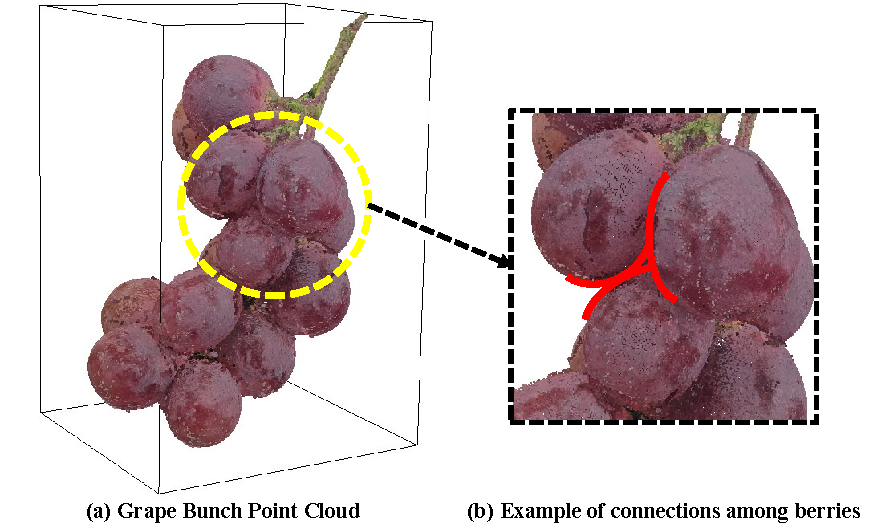
\includegraphics[width=1\textwidth]{figures/Figure5.pdf}
    \caption{Example of berry connection in a bunch (in the case of Red Grape). The red line in the figure shows the characteristics: multiple curves of different depths intersect each other}
    \label{fig:raw2}
\end{figure}

In this paper, SoftGroup \citep{vu_softgroup_2022} was selected for bunch point cloud segmentation after comparing different deep learning-based point cloud instance segmentation models. 
SoftGroup used a two step approach: 
(1) the point-by-point prediction U-Net was used to capture the detailed geometric characteristics between points. 
(2) a threshold score was used to judge the boundary of the point to avoid point category misclassification. 
Therefore, it is suitable for use in a bunch where there is a tight connection between the berries.

In order to train and validate SoftGroup, each berry and stem in the bunch point cloud obtained in Section~\ref{sec:212} was labeled at the instance-level (Fig.~\ref{fig:raw11}). 
This paper collected and labeled eight bunches for each of the four species (in total 32 bunches). 
Five grape bunches per grape specie (in total 20) were randomly selected and used as training samples. The remaining three bunches were used for validation.

% figure 11
\begin{figure}[hbt!]
    \centering
    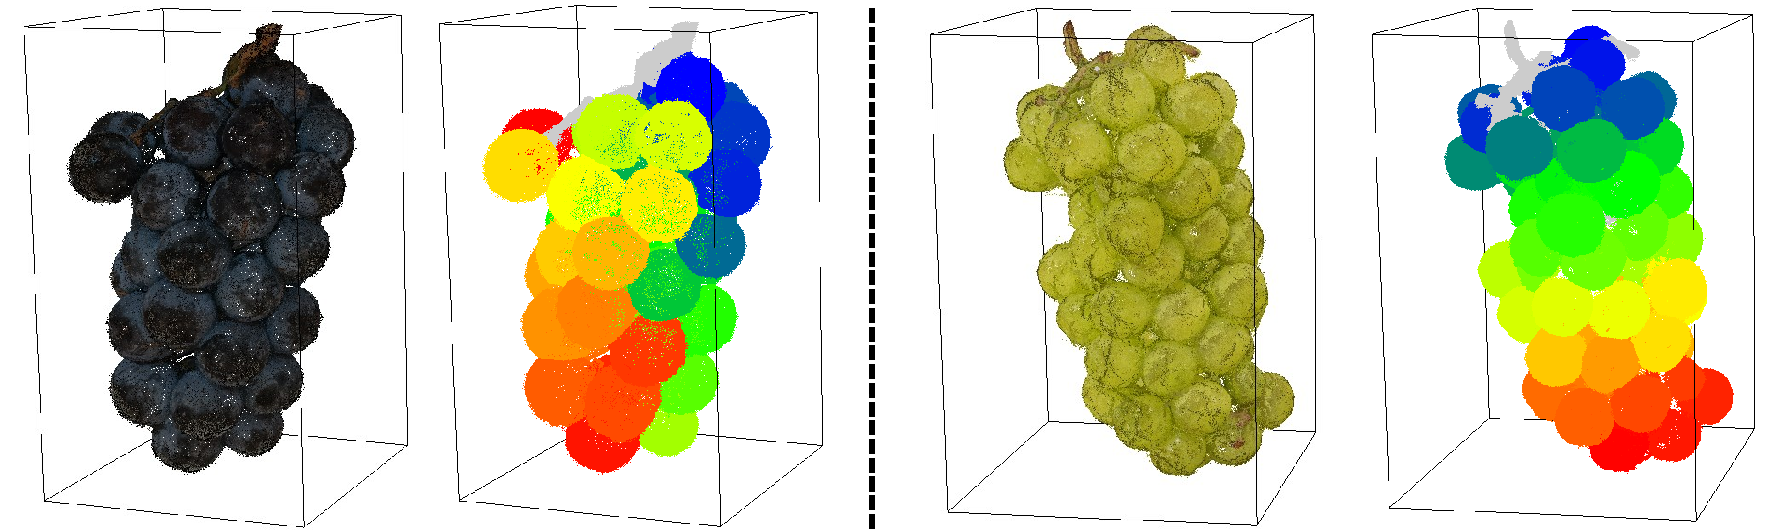
\includegraphics[width=1\textwidth]{figures/Figure6.pdf}
    \caption{Example of instance-level labeling of a bunch point cloud: each berry has a unique instance label, as shown by different colors of point sets}
    \label{fig:raw11}
\end{figure}

\subsection{Self-Supervised Point Cloud Completion}

The self-supervised training-based berry point cloud completion was used to predict their complete 3D model. 
Self-supervised learning is a way of training a model without annotations by clustering the data in unsupervised manners. 
The following section summarizes the self-supervised strategy for the paired training data. It is followed by a description of the grape completion network, GrapeCPNet (Figure~\ref{fig:raw3}).

% figure 3
\begin{figure}[hbt!]
    \centering
    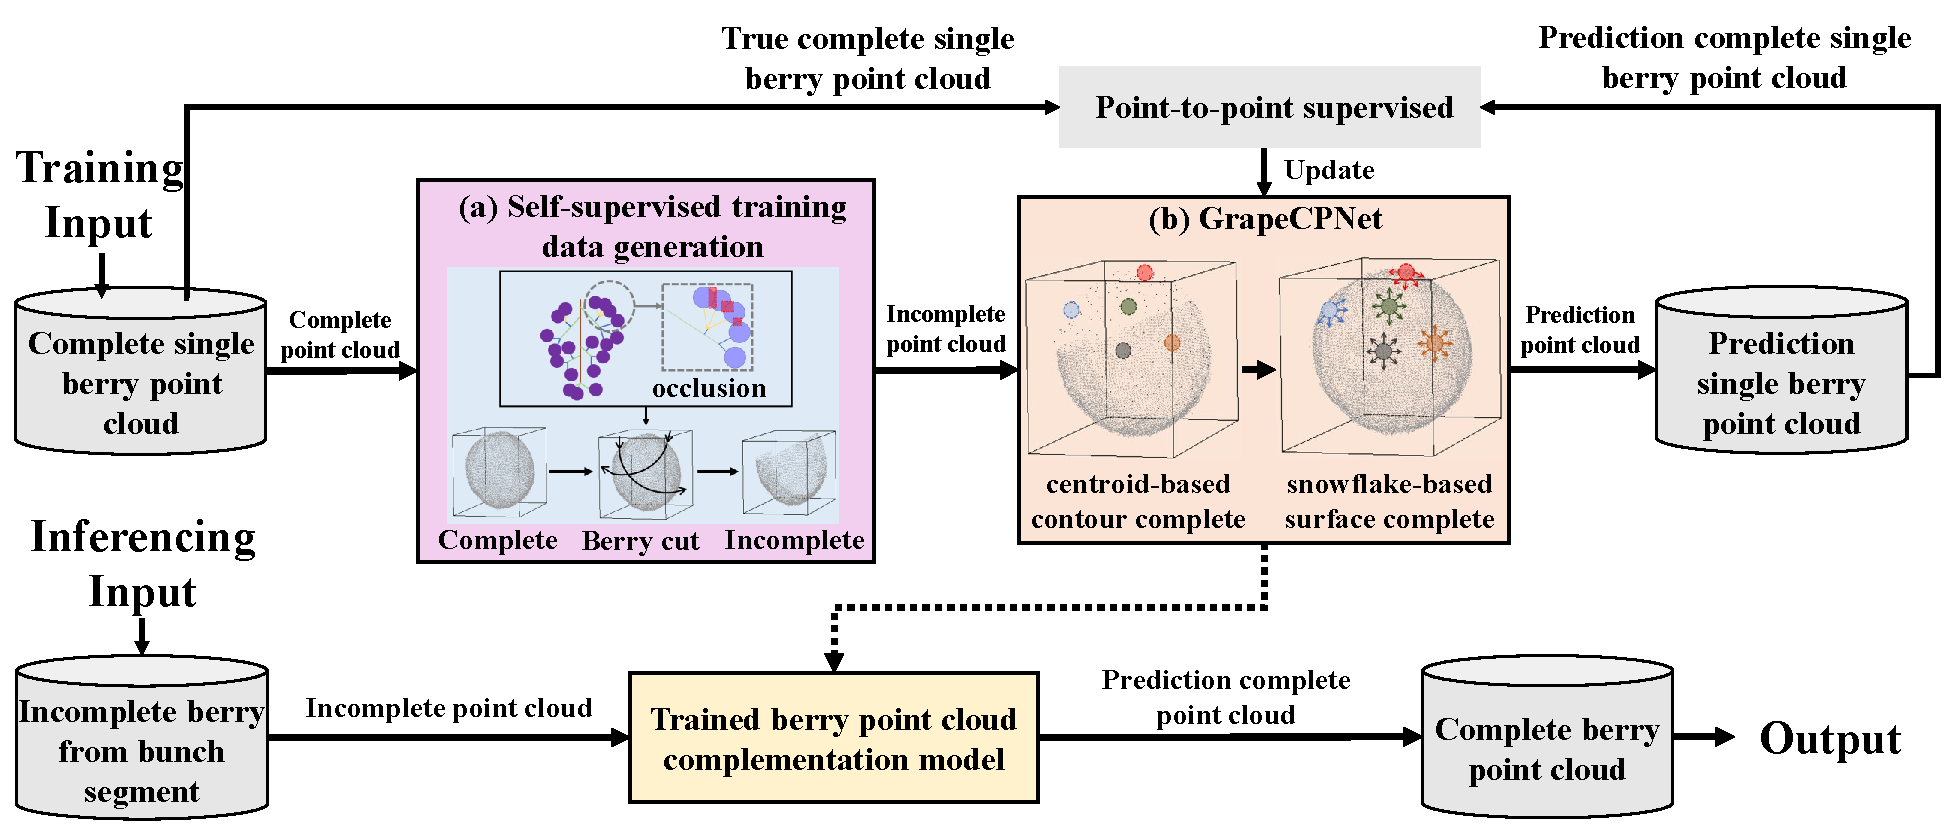
\includegraphics[width=1\textwidth]{figures/Figure7.pdf}
    \caption{Flowchart of the self-supervised berry point cloud completion, including model training and model inferencing (application) phases. In the training phase, the paired incomplete training data was generated from the complete single berry point cloud, then GrapeCPNet was trained using self-supervised methods without manual annotation. In the application phase, the incomplete berry point cloud is input to the trained model to obtain a complete prediction berry.}
    \label{fig:raw3}
\end{figure}

\subsubsection{Self-supervised training data generation}
\label{sec:berrycut}

Supervised point cloud completion training requires the incomplete-complete data pairs of the same object to build a mapping relationship. 
In this paper, the complete grapes were obtained by single berry reconstruction (Section~\ref{sec:212}) and were used as ground truth, while the incomplete grapes were cut from the complete grapes following characteristic of occlusion and were used as training inputs. 
This data pair generation strategy alleviated the data annotation efforts. The common incomplete characteristics of the berry are shown in Figure~\ref{fig:raw4}.
Based on the incomplete characteristics, we developed a selection method to generate the incomplete berry point cloud from the complete berry point cloud .

% figure 4
\begin{figure}[hbt!]
    \centering
    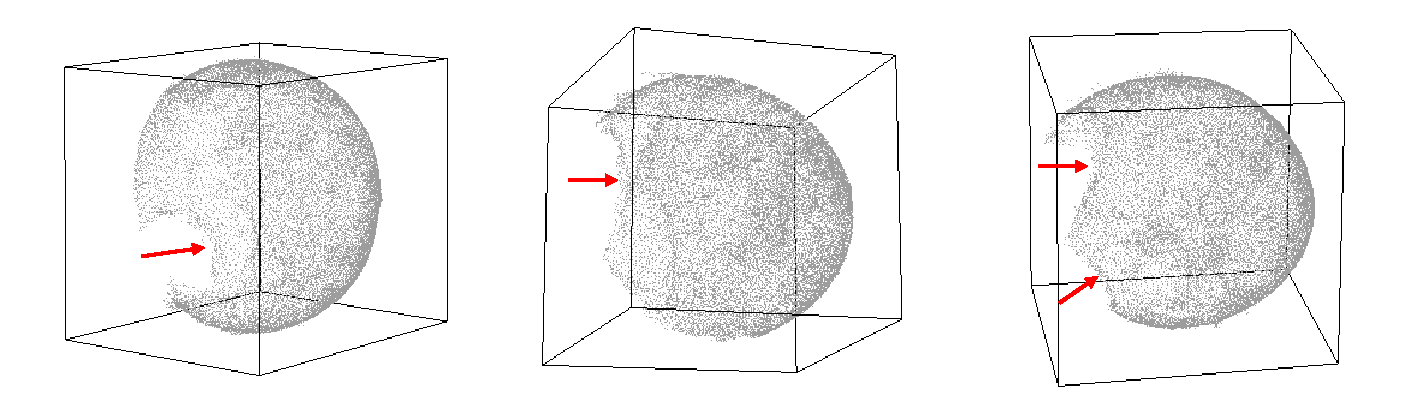
\includegraphics[width=1\textwidth]{figures/Figure8.pdf}
    \caption{Example of different perspectives of an incomplete berry point cloud segmented from the bunch. The edge of the absence shows multiple segments connected by circular curves, as shown by the red arrows}
    \label{fig:raw4}
\end{figure}

The pseudo-code of our proposed algorithm is shown in Algorithm \ref{alg:1}. 
The inputs include a single complete berry point cloud and the maximum number of selection areas (5 in this paper). 
The output is a selected incomplete berry point cloud. First, the single complete berry point cloud was normalized and centralized (Fig.~\ref{fig:raw12}a). 
Second, randomly select the number of cuts, with a maximum of five cuts as specified in this paper. 
Then, for each loop of selection, a 3D sphere model was generated in the space to collide with the berry point cloud, and the collision portion was removed to complete the operation. 
The maximum center and radius parameters of the 3D sphere model were manually set according to the berry size. 
In this paper we set a maximum of 0.75 for the center offsets and 0.25 for the radius offsets. 
Continue the previous selection looping until the limits are met. The selected incomplete point cloud was saved from each loop as training data (Fig.~\ref{fig:raw12}b). 

% algorithm 1
\begin{algorithm}
    \caption{The selection method for generating training data of incomplete berries}
    \label{alg:1}
    \KwData{$P_C$ \tcp{one complete berry point cloud}}
    \KwData{$n$ \tcp{generate incomplete berries number}}
    \KwResult{$P_{\text{output}} = \{P_{o_i} \mid i = 1, \cdots, n\}$ \tcp{incomplete berry point cloud sets} }
    
    $\hat{P}_C \gets \text{Normalize}(\text{Translate}(P_C))$ \tcp{center to $(0,0,0)$, range to $[-0.5m, 0.5m]$}
    \For{$i = 0 \to n$}{
        set $m = \text{random}\{1,2,3,4,5\}$ \tcp{select incomplete single berry $m$ times}
        $P_{o_i} \gets copy(\hat{P}_C)$ \tcp{initialize one output}
        \For{$j = 0 \to m$}{
            set $O = \{(x_o, y_o, z_o) \mid x, y, z \in \text{random}[-0.75, 0.75]\}$ \tcp{center} 
            set $R = \text{random}[0.25, 0.75]$ \tcp{radius}
            set $M_S \gets \text{sphere}(O, R)$ \tcp{generate sphere model}
            $P_{o_i} = P_{o_i} - P_{o_i} \cap M_S$ \tcp{remove overlap with sphere model}
        }
        $P_{\text{output}_i} \gets P_{o_i}$ \tcp{add to output set}
    }
\end{algorithm}

% figure 12
\begin{figure}[hbt!]
    \centering
    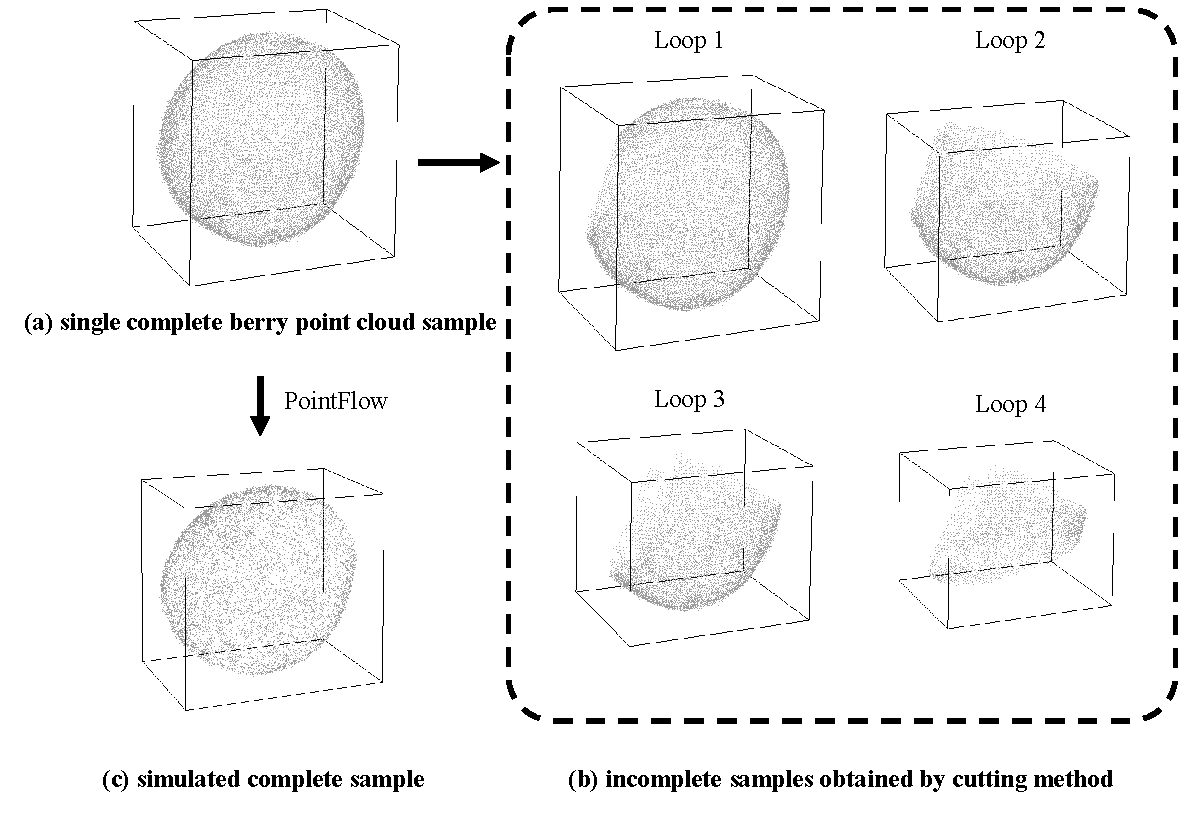
\includegraphics[width=1\textwidth]{figures/Figure9.pdf}
    \caption{Example of dataset composition for the self-supervised training-based method of the berry point cloud completion network.}
    \label{fig:raw12}
\end{figure}

For model training, 36 complete berry were collected for each of the four species of grape (in total 144). 
To further expand the data quantity, based on the single complete berry point cloud obtained by reconstruction, this paper uses the PointFlow \citep{yang_pointflow_2019}, a point cloud generation model to generate the simulated samples (Fig.~\ref{fig:raw12}c). 
Then, 500 complete berry point clouds are generated from PointFlow method. 
Thus, a total of 644 complete samples are obtained. 
Each complete berry point cloud has 5 incomplete berry point clouds corresponding to it, and a total of 3220 training data pairs are obtained. 
For the training and testing of the model, this paper divides the dataset according to a ratio close to 70-30\%, with a total of 450 complete berry point clouds (2250 training data pairs) to train the network and 194 complete berry point clouds (970 testing data pairs) to test.

For the model inference validation, from the 12 testing grape bunches of the berry instance,  one bunch was randomly selected per grape specie (in total 4 bunches), refer to (Section~\ref{sec:22}). 
For each bunch, 27 berries were randomly selected, yielding a total of 108 incomplete berries for testing the completion network inference validation. 
The labels of these berries (Section~\ref{sec:212} \& Fig.~\ref{fig:raw9}c), were used as ground truth.

\subsubsection{GrapeCPNet}

Since the entire contour of the incomplete berry is missing, the model is required to have the ability to predict the incomplete part based on the visible part and make the prediction part fit the real berry surface and avoid detail distortion. 
This paper combines the centroid-based sparse completion structure of PoinTr \citep{yu_pointr_2021} with the diffusion-based dense completion structure of SnowFlakeNet \citep{xiang_snowflakenet_2021}. 
Based on the characteristics of the berry, it has two parts: contour completion and surface completion. The network structure is shown in Figure~\ref{fig:raw5}.

% figure 5
\begin{figure}[hbt!]
    \centering
    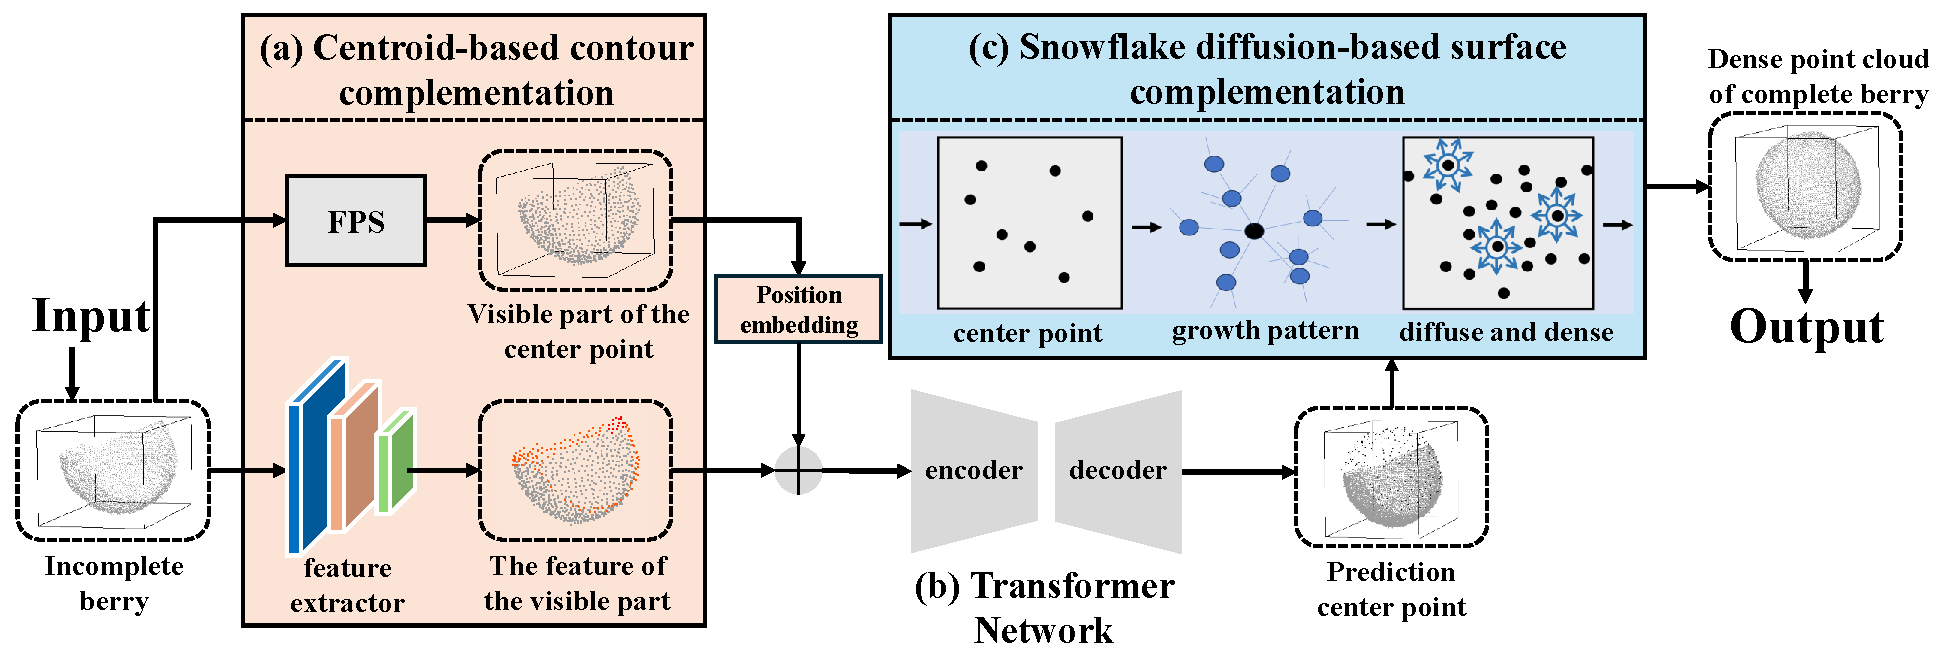
\includegraphics[width=1\textwidth]{figures/Figure10.pdf}
    \caption{GrapeCPNet structure. (a) Centroid-based completion and (b) Transformer network for contour completion of incomplete berry, using sparse point cloud to determine the entire shape; (c) Snowflake diffusion-based completion for dense surface completion to obtain final prediction.}
    \label{fig:raw5}
\end{figure}

{\raggedright\textbf{(a) Centroid-based berry contour completion}}

The visible portion of the incomplete berry belongs to a part of a sphere or ellipsoid, characterized by a distinctly spherical surface. 
In addition, the point cloud is unstructured data, unstructured and dense, resulting in features that cannot be effectively extracted. 
Based on the above analysis, this paper utilizes the centroid set of the visible part to infer the centroid set of the invisible part. 
Specifically, GrapeCPNet uses centroid-based feature extraction in PoinTr \citep{yu_pointr_2021} to accomplish berry point cloud contour completion. The process is described below: 

Assume that the set of incomplete berry point cloud as input to the network is represented as $P_{partial}=\{p_i \mid i=1, \cdots, m \}$, where $p_i=(x_i,y_i,z_i)$ denotes a point in 3D space and $m$ denotes the number of points. 
The berry point cloud completion task aims to output the complete berry point set $P_{complete}=\{p_i \mid i=1, \cdots, n\}$, where $n$ denotes the number of points of the output, and $n > m$, thereby it can represent the complete 3D morphology of the berry.

After the incomplete berry point cloud set $P_{partial}=\{p_i \mid i=1,\cdots,m\}$ was fed into the network, it was firstly down-sampled to a fixed number of points $M$ ($M$ is often less than $m$, in this paper, $M$ is set to 2048) through the farthest point sampling (FPS) to obtain the center point set $P_{partial-center}=\{p_i \mid i=1, \cdots, M\}$ of the visible part of the berry. 
This set was used as a ``representative'' to avoid huge computational effort while characterizing the complete morphology of the visible part.

Then, the 3D convolutional neural networks DGCNN \citep{wang_dynamic_2019} and MLP \citep{tolstikhin_mlpmixer_2021} are used to obtain the local structural features of each point $p_i$ in the center point set, as shown in Equation~(\ref{eq:2}).

\begin{equation}
    F_i = F_{i}^{'} + \varphi(p_i)
    \label{eq:2}
\end{equation}

{\raggedright where, $F_{i}^{'}$ denotes the feature around $p_i$ obtained by DGCNN, which is the local feature of the point in the point cloud; and $\varphi(p_i)$ denotes the position information of $p_i$ obtained by MLP, which is the global feature of the point.}

{\raggedright\textbf{(b) Transformer network}}

Since the $\varphi = \{ \varphi(p_i) \mid i=1, \cdots, M \}$ contains the relative position information of each point, it can be used as the position embedding and the serialized feature $F = \{F_i \mid i=1, \cdots, M \}$ was fed into the geometrically-aware Transformer \citep{vaswani_attention_2017} based encoder. 
The process is Equation~(\ref{eq:3}).

\begin{equation}
    V = T_e(F)
    \label{eq:3}
\end{equation}

{\raggedright where, $T_e$ denotes the encoder of the Transformer and $V=\{V_i |i=1, \cdots, M\}$ denotes the encoded feature. 
Next, the predicted centroid point set of the missing part was output by the decoder, and the process as Equation~(\ref{eq:4}).}

\begin{equation}
    P_{pred-center} = T_d(V)
    \label{eq:4}
\end{equation}

{\raggedright where, $T_d$ denotes the decoder of the Transformer, $P_{pred-center}=\{p_i \mid i=1,\cdots,N\}$ denotes the predicted centroid point set, and $N$ denotes the number of points in the set. 
Through the above steps, the set of center points of the complete berry can be initially obtained, which was the result of sparse contour completion.}

{\raggedright\textbf{(c) Snowflake diffusion-based berry surface completion}}

The results of the contour completion can determine the overall 3D morphology, however, the density of this sparse point cloud requires the model to capture the detailed surface geometry changes between the points to prevent distortion. 
Therefore, this paper utilizes the snowflake diffusion-based generation method to regard each point in the contour completion as the center point of the local region. 
Its diffusion is based on the centroid points and generates further at the generated location, densification by point-to-point splitting. 
Specifically, as follows:

First, GrapeCPNet sets each point $p$ of the sparse complement $P_{pred-center}=\{p_i \mid i=1,\cdots,N\}$ as a ``seed point''. 
Then, $P_{pred-center}$ was fed into multiple SPD \citep{xiang_snowflakenet_2021} connected serially of SnowFlakeNet, which are used to realize point splitting and generation. 
On the one hand, the SPD diffuses from the center point in a tree structure around, revealing the detailed geometric structure of the local region. 
This method effectively represents the surface geometric features composed between the points in the localized region of the berry. 
On the other hand, the iteration of multiple point splitting steps delivers information from each one to the next one. 
This approach effectively characterizes the curvature changes on the surface of the berry. The process is Equation~(\ref{eq:5}).

\begin{equation}
    P_{i+1} = SPD(P_i)
    \label{eq:5}
\end{equation}

{\raggedright where, $P_i$ denotes the input point cloud of the $i^{\text{th}}$ SPD, $P_{i+1}$ denotes the output point cloud of the $(i+1)^{\text{th}}$ SPD, and $P_0=P_{pred-center}$. 
In this paper, when $i=2$ (an empirical value), the final predicted dense point cloud on the surface of the complete berry $P_3=P_{complete}$ was output and $P_{complete}=\{p_i \mid i=1,\cdots,n\}$.}

Through the above steps, the complete 3D point cloud model of the berry can be obtained after contour completion and surface completion of GrapeCPNet.

\subsection{Phenotypic Traits Calculation and Validation}

To describe the 3D morphology of berries, this paper used ellipsoidal surface fitting with three axes, for the completed berry point cloud (Fig.~\ref{fig:raw16}).

% figure 16
\begin{figure}[hbt!]
    \centering
    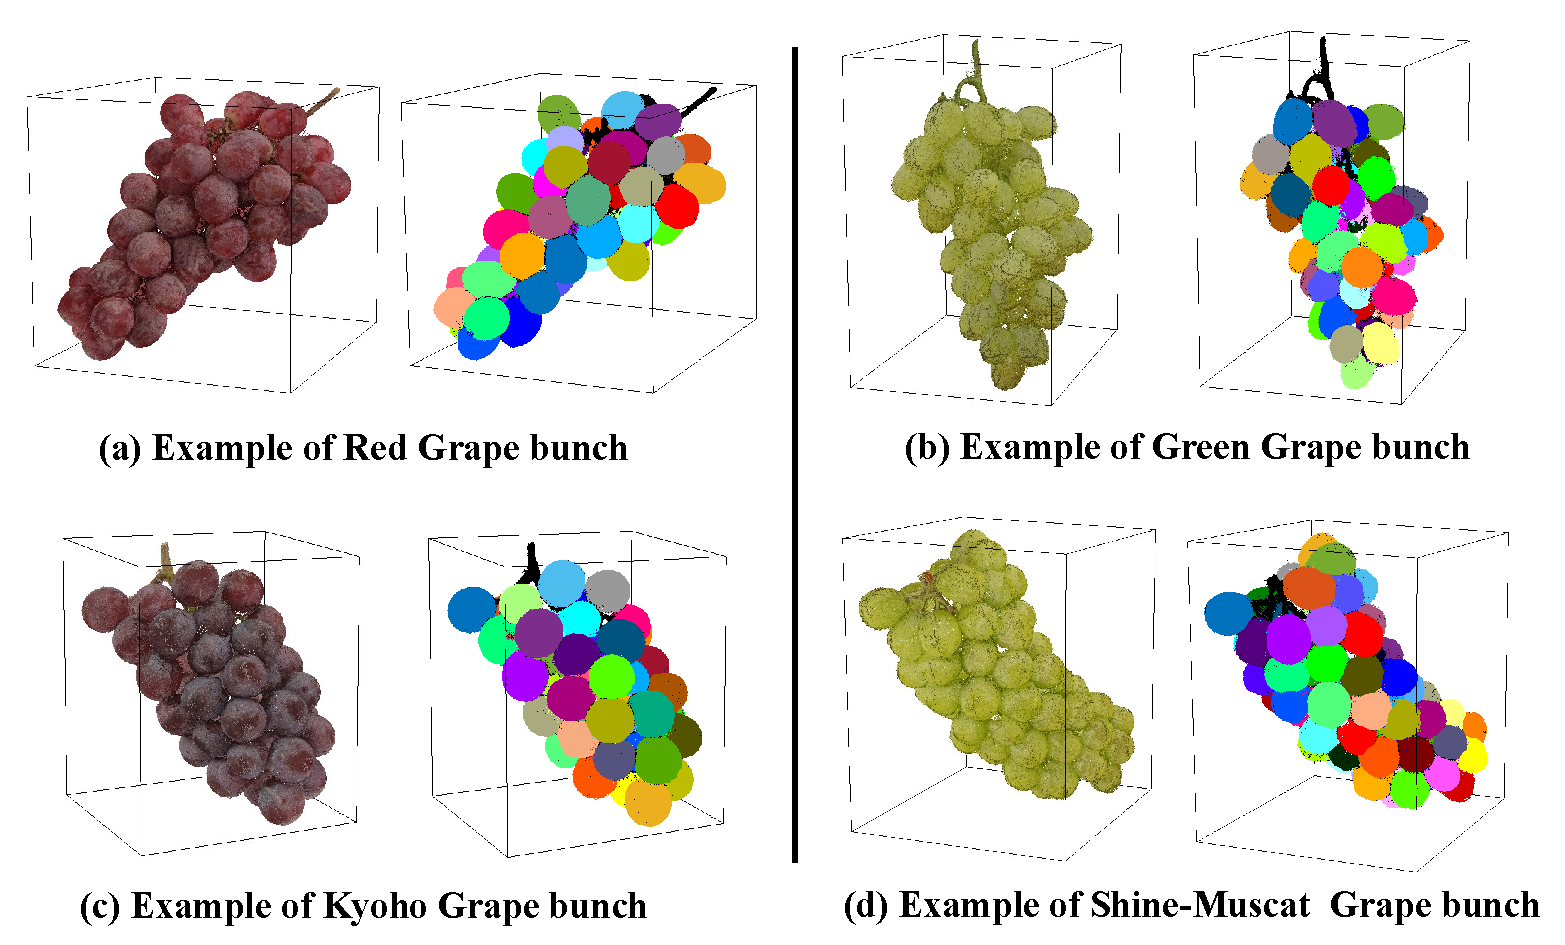
\includegraphics[width=1\textwidth]{figures/Figure11.pdf}
    \caption{Example of \deleted{visualization of the predicted complete }berry point cloud fitted to \replaced{its ellisoid surface}{the surface of an ellipsoid}.}
    \label{fig:raw16}
\end{figure}

% figure 7 -> removed

Suppose the point cloud of \replaced{a}{the} complete berry is denoted as $P_{complete}=\{P_i \mid i=1, \cdots,n\}$, where $p_i=(x_i,y_i,z_i)$ denotes a point in the 3D space, and $n$ denotes the number of points. 
In this paper, it is fitted to an ellipsoid surface with three unequal long axes by the least squares method, and the function is shown in Equation~(\ref{eq:6}).

\begin{equation}
    \frac{(x-x_0)^2}{a^2} + \frac{(y-y_0)^2}{b^2} + \frac{(z-z_0)^2}{c^2} = 1
    \label{eq:6}
\end{equation}

{\raggedright where, $(x,y,z)$ denotes a point on the ellipsoid surface, $(x_0,y_0,z_0)$ denotes the coordinates of the ellipsoid center point, and $a$, $b$, $c$ are the half-long, half-middle, and half-short axes, respectively (assuming that $a>b>c>0$). }

Thus, the values of $a$, $b$, $c$ can represent the berry radius parameters. 
At the same time, the volume of the berry can be calculated as shown in Equation~(\ref{eq:7}).

\begin{equation}
    V=\frac{4}{3} \pi a b c
    \label{eq:7}
\end{equation}

To validate the accuracy of extracted morphological traits, the 12 validation bunches \added{with 108 berry samples} were \replaced{selected. The berries were first scanned while still attached to bunch (Fig.~\ref{fig:raw9}a2). After instance segmentation, these scans of each berry are incomplete caused by occlusion. We then applied our proposed self-supervised completion method to get completion predictions. Finally get ellipsoidal surface fitting results as prediction values. }{ used after instance berry segmentation and berry completion (refer to Section~\ref{sec:22})} 
\deleted{The radius and volume of the 108 samples were calculated.} 
For ground truth measurement, \replaced{we separated berries from the bunch to get complete scans of corresponding berry (Fig.~\ref{fig:raw9}b1). Then applied the ellipsoidal surface fitting to these completely scans. }{we used the values of the radius and volume of the individual complete berry from the completed point clouds.}

\subsection{Evaluation Metrics}

In this paper, the metrics for the bunch segmentation, berry completion, berry counting, and the radius and volume calculation were used for evaluating the performance of our analysis pipeline.

\subsubsection{Berry instance segmentation}
\label{sec:251}
In this paper, we used average precision AP as the evaluation metric for berry instance segmentation, similar to the original paper of \added{SoftGroup} \citep{vu_softgroup_2022}. The average APs with IoU (Intersection over Union) ranging from 50\% to 95\% in steps of 5\% were used and noted as \replaced{mAP@[.5:.95]}{AP@50:5:95}.

\subsubsection{Berry self-supervised completion}

In this paper, we use the chamfer distance (CD-distance) and F-Score to measure the effect of berry completion,  similar to the original paper of \citet{yu_pointr_2021}. 
For each sample, the chamfer distance $d_{CD}$ between the predicted point set $P$ and the true point set $G$ was calculated as shown in Equation~(\ref{eq:8})

\begin{equation}
    d_{CD}(P, G) = \frac{1}{|P|} \sum_{p \in P} \min_{g \in G} \|p - g\|_2^2 + \frac{1}{|G|} \sum_{g \in G} \min_{p \in P} \|g - p\|_2^2
    \label{eq:8}
\end{equation}

{\raggedright where, $|P|$ denotes the number of points of $P$, $|G|$ denotes the number of points of $G$, and $\|p - g\|$ denotes the distance between $p$ and $g$. 
It can be seen that the chamfer distance represents the sum of the average closest distance from the point in $P$ to the point in $G$ and the average closest distance from the point in $G$ to the point in $P$. Where the L1 norm was used to calculate the closest distance between two points.}

The F-Score measured the similarity between $P$ and $G$ by the harmonic mean between Precision and Recall (Eq.~\ref{eq:9}). 
Precision (Eq.~\ref{eq:10}) is the percentage of predicted points within a certain distance from the truth point, i.e. the accuracy of the prediction. Recall (Eq.~\ref{eq:11}) is the percentage of ground truth points within a certain distance from the predicted point, i.e. the completeness of the prediction. 

\begin{equation}
    F\text{-Score}(d) = \frac{2 \times \text{Precision}(d) \times \text{Recall}(d)}{\text{Precision}(d) + \text{Recall}(d)} 
\label{eq:9}
\end{equation}


\begin{equation}
    \text{Precision}(d) = \frac{1}{|P|} \sum_{p \in P} \left[ \min_{g \in G} \|p - g\| < d \right]\\
\label{eq:10}
\end{equation}

\begin{equation}
    \text{Recall}(d) = \frac{1}{|G|} \sum_{g \in G} \left[ \min_{p \in P} \|g - p\| < d \right]
\label{eq:11}
\end{equation}

{\raggedright The distance threshold $d$ was set to $0.01m$. Given that the point cloud was initially normalized to the range $[-0.5m, 0.5m]$. 
From the above Equation, the higher the F-Score the better the match between the two point sets.}

To verify the efficiency of GrapeCPNet, we compared it to other point cloud completion networks: PoinTr \citep{yu_pointr_2021} SnowFlakeNet \citep{xiang_snowflakenet_2021}, TopNet \citep{tchapmi_topnet_2019}, and GRNet \citep{xie_grnet_2020}.

\subsubsection{Phenotypic traits calculation}
\label{sec:253}
To evaluate the efficiency of the number of berry statistics and the calculation of berry radius and volume, the MAE (Mean Absolute Error) and the coefficient of determination $R^2$ (R-Square) are used to calculate the error between the prediction value and the true value of the sample.

\begin{align}
    \text{MAE} &= \frac{1}{m} \sum_{i=1}^{m} |y_i - \hat{y}_i| \tag{12}\\
    R^2 &= 1 - \frac{\sum_{i=1}^{m} (\hat{y}_i - y_i)^2}{\sum_{i=1}^{m} (\bar{y}_i - y_i)^2} \tag{13}
\end{align}

{\raggedright where, $m$ is the number of samples, $y_i$ is the true value of the $i^{\text{th}}$ sample, $\hat{y}_i$ is the prediction value, and $\bar{y}_i$ represents the mean of all true values. 
The lower the MAE, the closer the prediction value is to the true value. The values of $R^2$ range between 0 and 1, and the closer it is to 1 means the better the fit with the predicted values.}

\section{Results}

To validate the efficiency of our method, the experiments were conducted on each component separately, including the result of bunch point cloud segmentation, the result of berry point cloud completion based on self-supervised training, and the result of obtaining the phenotypic traits.

\subsection{Berry Instance Segmentation Results}
\label{sec:insegresults}

\deleted{The bunch point cloud segmentation results are summarized in Table~\ref{tbl:3} }. 
% table 3
% \begin{table}[h]
%     \centering
%     \caption{Instance berry segmentation results from whole bunch}
%     \begin{tabular}{ccc}
%         \hline
%         \textbf{Class} & \textbf{mAP@[.5:.95]} \\
%         \hline
%         Berry & 0.995 \\
%         Stem & 0.941 \\
%         \hline
%     \end{tabular}
%     \label{tbl:3}
% \end{table}
\deleted{As can be seen from Table~\ref{tbl:3}, The value of the point cloud instance segmentation for the berry category is over 99\%, which shows a high accuracy of the berry segmentation from the bunch.}

\added{The mAP@[.5:.95] values of berry and stem class are 0.995 and 0.941, respectively, which }showed a high accuracy of the berry segmentation from the bunch.
\added{Since mAP@[.5:.95] is a strict evaluation metric, it represents the mean values of Average Precision (AP) scores calculated from AP50 to AP95 at 5\% IoU intervals}.
\added{Compared to other studies, \citet{ni_threedimensional_2021} reported that their proposed segmentation network achieved a mAP@[.5:.95] of 0.877 on their testing dataset, while \citet{du_instance_2023} achieved a mAP[.5:.95] of 0.657 and an AP50 of 0.952.}
\added{In our study, the AP50 value exceeded 0.999, with both recall and precision values at this level also over 0.999.}
\added{When compared to traidtional berry semgnetation algorithms, \citet{rose_automated_2016} reported a mean recall of 0.776 and precision of 0.978;}
The results of four fresh grapes for bunch point cloud segmentation are visualized in Fig.~\ref{fig:raw13}.
\added{According that figure, we can also see an almost perfect instance berry segmentation results.}

% figure 13
\begin{figure}[hbt!]
    \centering
    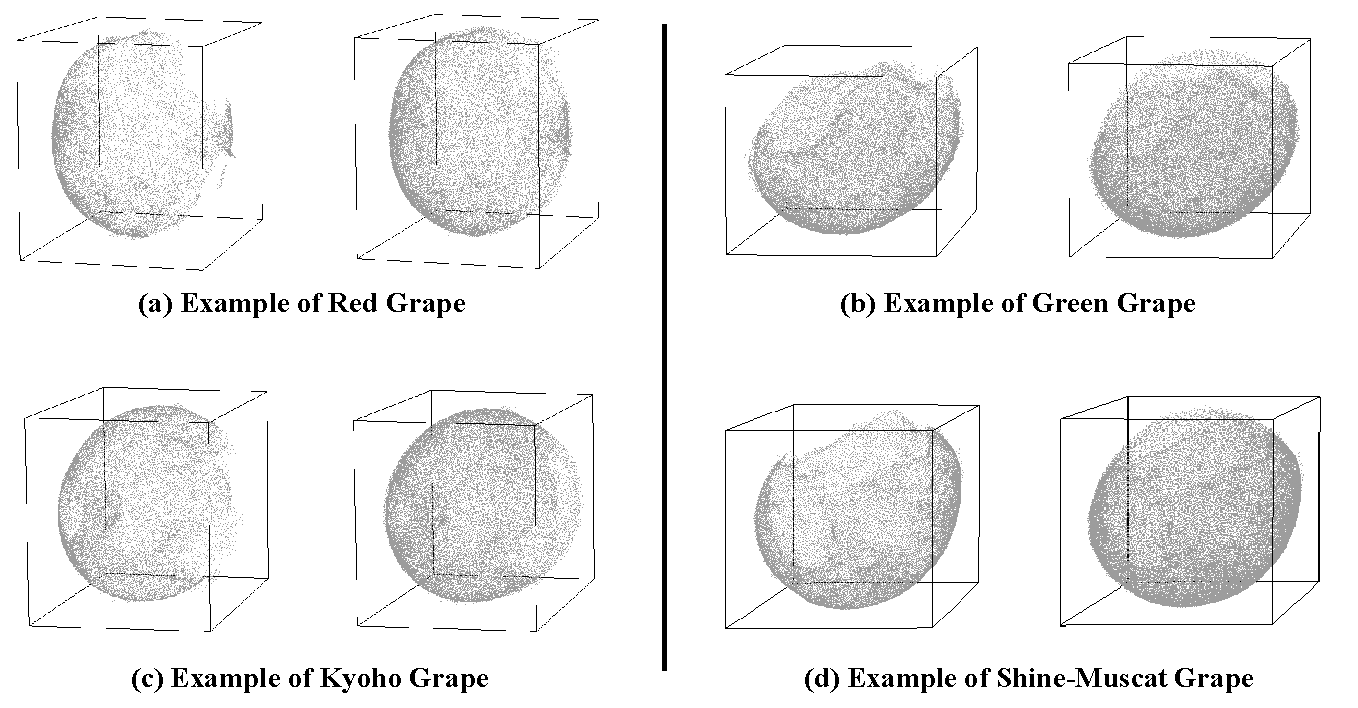
\includegraphics[width=1\textwidth]{figures/Figure12.pdf}
    \caption{Segmentation results of the bunch of four species of fresh grape, the stems point cloud and the noise point cloud are set to black, and the different color point sets indicate the point clouds of different berry instances obtained.}
    \label{fig:raw13}
\end{figure}

\subsection{Berry Self-Supervised Completion Results}
\label{sec:32}

The berry point cloud completion experiments are divided into two parts according to the different phases of the network: 
the results of the self-supervised training \added{(Test)} and the results of the practical application \added{(Inference)}.
\replaced{As}{The experimental results of GrapeCPNet compared to other point cloud completion algorithms are} shown in Table~\ref{tbl:4}, 
GrapeCPNet achieves the best results under the self-supervised training method in both the training phase and the application phase, better than the comparative algorithms. Fig.~\ref{fig:raw14} visualizes the shape completion result of GrapeCPNet on the incomplete berry segmented from the bunch in the application phase.

% table 4
\begin{table}[h]
    \centering
    \caption{\replaced{Comparing proposed method with}{Experimental results of} different completion networks \deleted{based on self-supervised training} for berry point cloud. Best performing results are visualized in bold.}
    \begin{tabular}{cccccc}
        \hline
        \textbf{Model} & \textbf{DataSet} & \textbf{$d_{CD}$ (mm) $\downarrow$} & \textbf{Precision $\uparrow$} & \textbf{Recall $\uparrow$} & \textbf{F-score $\uparrow$} \\
        \hline
        \multirow{2}{*}{\makecell{PoinTr \\ \citep{yu_pointr_2021}}} & Test & 9.036 & 0.721 & 0.705 & 0.713 \\
        \cline{2-6}
        & Inference & 10.542 & 0.623 & 0.601 & 0.612 \\
        \hline
        \multirow{2}{*}{\makecell{SnowFlakeNet \\ \citep{xiang_snowflakenet_2021}}} & Test & 11.235 & 0.512 & 0.534 & 0.521 \\
        \cline{2-6}
        & Inference & 12.384 & 0.415 & 0.423 & 0.419 \\
        \hline
        \multirow{2}{*}{\makecell{TopNet \\ \citep{tchapmi_topnet_2019}}} & Test & 23.019 & 0.201 & 0.200 & 0.201 \\
        \cline{2-6}
        & Inference & 31.880 & 0.155 & 0.154 & 0.154 \\
        \hline
        \multirow{2}{*}{\makecell{GRNet \\ \citep{xie_grnet_2020}}} & Test & 19.240 & 0.402 & 0.392 & 0.397 \\
        \cline{2-6}
        & Inference & 21.250 & 0.365 & 0.363 & 0.364 \\
        \hline
        \multirow{2}{*}{\makecell{GrapeCPNet \\ (Ours)}} & Test & \textbf{8.315} & \textbf{0.729} & \textbf{0.772} & \textbf{0.751} \\
        \cline{2-6}
        & Inference & \textbf{9.158} & \textbf{0.685} & \textbf{0.696} & \textbf{0.689} \\
        \hline
    \end{tabular}
    \label{tbl:4}
\end{table}

% figure 14
\begin{figure}[hbt!]
    \centering
    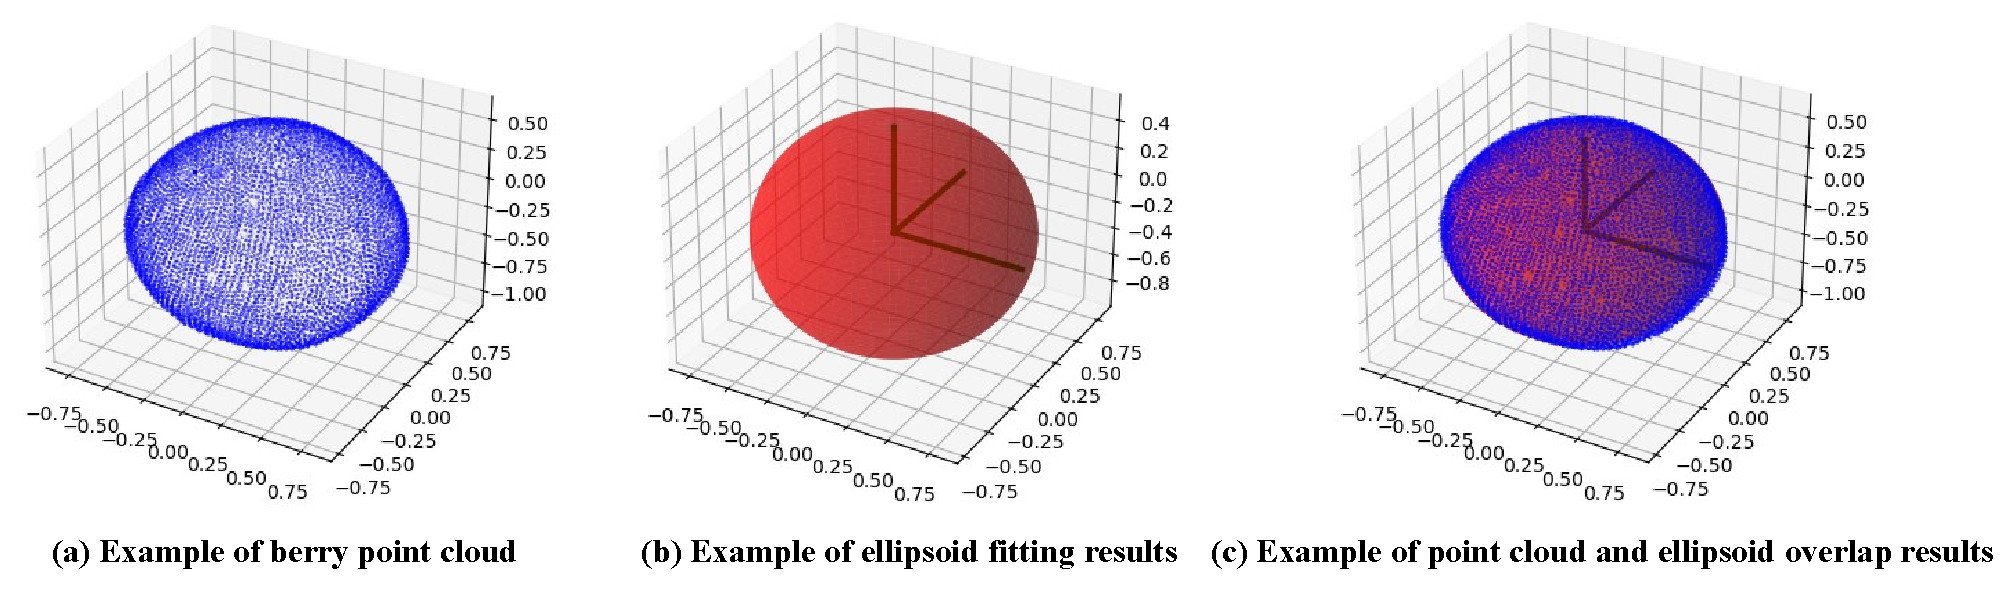
\includegraphics[width=1\textwidth]{figures/Figure13.pdf}
    \caption{Example of four fresh grape berry point cloud completion results: in subfigures a-d, the left side shows \replaced{incomplete berry while}{the incomplete berry point cloud obtained from the segmentation of the bunch, and} the right side shows the completion results using \added{proposed} GrapeCPNet \deleted{under the self-supervised training-based method}.}
    \label{fig:raw14}
\end{figure}

The results of the ``Inference'' experiments are worse than those of the ``Test'' experiments for two main reasons.
First, there are differences between the dataset of the training phase and the application phase of self-supervised training, resulting in a drop in the accuracy. 
In addition, when evaluating the actual application efficiency of the model, the true value of the reconstructed complete point cloud of a single berry and the prediction value of the complemented point cloud suffer from the drop in the accuracy after aligning them. 
Through the above results, the experiments of berry point cloud completion based on self-supervised training reflected the efficacy of GrapeCPNet, meanwhile, this paper further validated the efficacy of the 3D phenotypic traits of grape by the proposed method.

\subsection{Phenotypic Traits Calculation Results}

The radius parameters were calculated by fitting the berry to the surface of an ellipsoid\deleted{, as shown in Figure~\ref{fig:raw16}}.
From Figure~\ref{fig:raw17}, it can be seen that the proposed method achieves an average $R^2$ of 0.86 \added{and average MAE of 0.608 mm} for the three axis lengths of the four species of grape. 
This result can be dissected as follows:

% figure 17
\begin{figure}[hbt!]
    \centering
    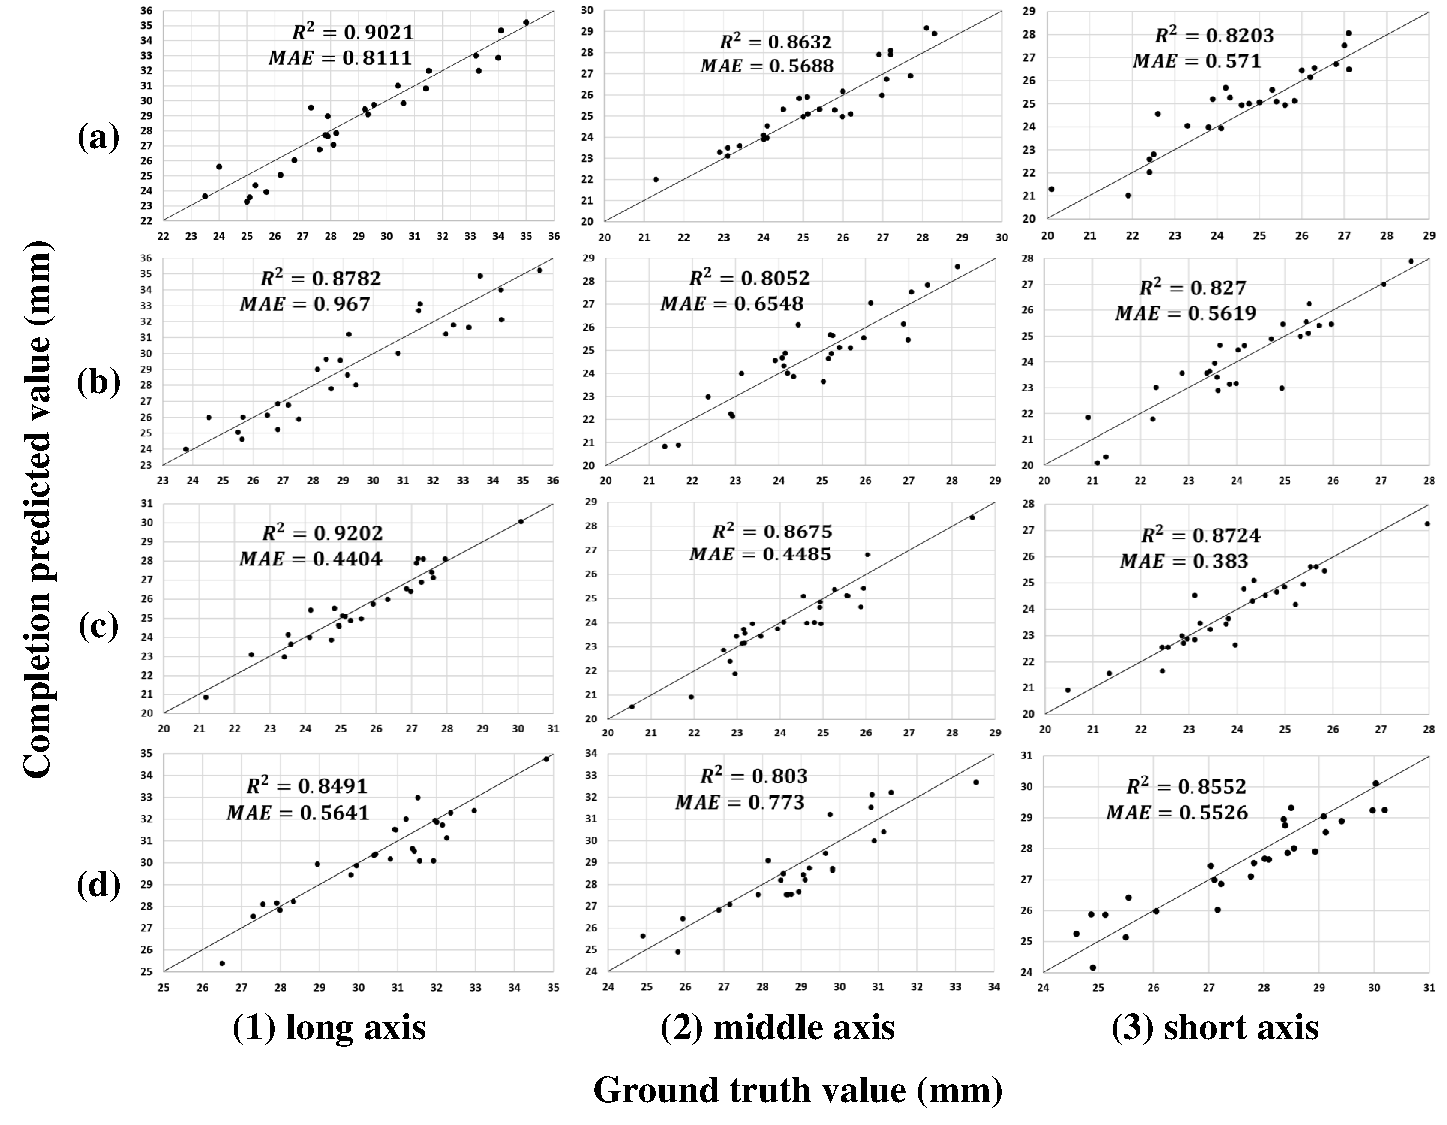
\includegraphics[width=1\textwidth]{figures/Figure14.pdf}
    \caption{Experimental results of axis length calculation for four species of fresh grape. From (a)-(d): Red Grape, Green Grape, Kyoho Grape, and Shine-Muscat Grape, \deleted{and from (1)-(3): the calculation of the long, middle, and short axis, }respectively. \added{The ground truth values are obtained by completely scanning berries that were separated from the bunch (Fig.~\ref{fig:raw9}b1); The predicted values are obtained from our proposed self-supervised completion method, which addresses incomplete scans of berries that occur due to occlusion while they were still attached to the bunch (Fig.~\ref{fig:raw9}a2).}}
    \label{fig:raw17}
\end{figure}

(1) The different species: Red Grape, Green Grape, Kyoho Grape, and Shine-Muscat Grape axis length prediction reached an average $R^2$ of 0.86, 0.84, 0.89, and 0.84, respectively. 
Among them, Kyoho Grape achieved the best results due to its spherical berries that are not too densely clustered and the lower difficulty in berry completion and morphology fitting. 
Secondly, Red Grape and Green Grape both present a typical ellipsoid shape, but the \replaced{Red}{latter} is less precise than the \replaced{Green}{former} due to its \replaced{larger}{greater} ratio of long axis to short axis, which provides a more complex presentation. 
\added{As also reported by \citet{schneider_predicting_2020}, the mean length-to-width ratio of Green Grape is 21.18mm to 18.75mm, while for Red Grape, it is 24.11mm to 18.41mm.}
Shine-Muscat Grape had the lowest precision, which was due to the fact that its berry grows tightly and occlude each other heavily, making it harder to accurately complete its shape.

(2) The different axis: the average $R^2$ of the four species of grape were 0.89, 0.83, and 0.84 for the long, middle, and short axis, respectively. 
It can be noted that the prediction accuracy of the long axis was significantly higher than that of the others, in which the $R^2$ of Red Grape and Kyoho Grape reached 0.90 and 0.92, respectively, achieving a high accuracy. 
This was due to the fact that in berry completion and fitting, the long axis is the easiest to determine, with less fitting errors compared to the other two axes.

In addition, based on the radius prediction results, the volume of all 108 berry samples was calculated in this paper, and the experimental results are shown in Figure~\ref{fig:raw18}.
For the berry volume calculation of the four species, the $R^2$ was 0.97, and the MAE was 0.3842 $cm^3$.
\deleted{Indicating a high precision for predicting the volume of the different species.}

% figure 18
\begin{figure}[hbt!]
    \centering
    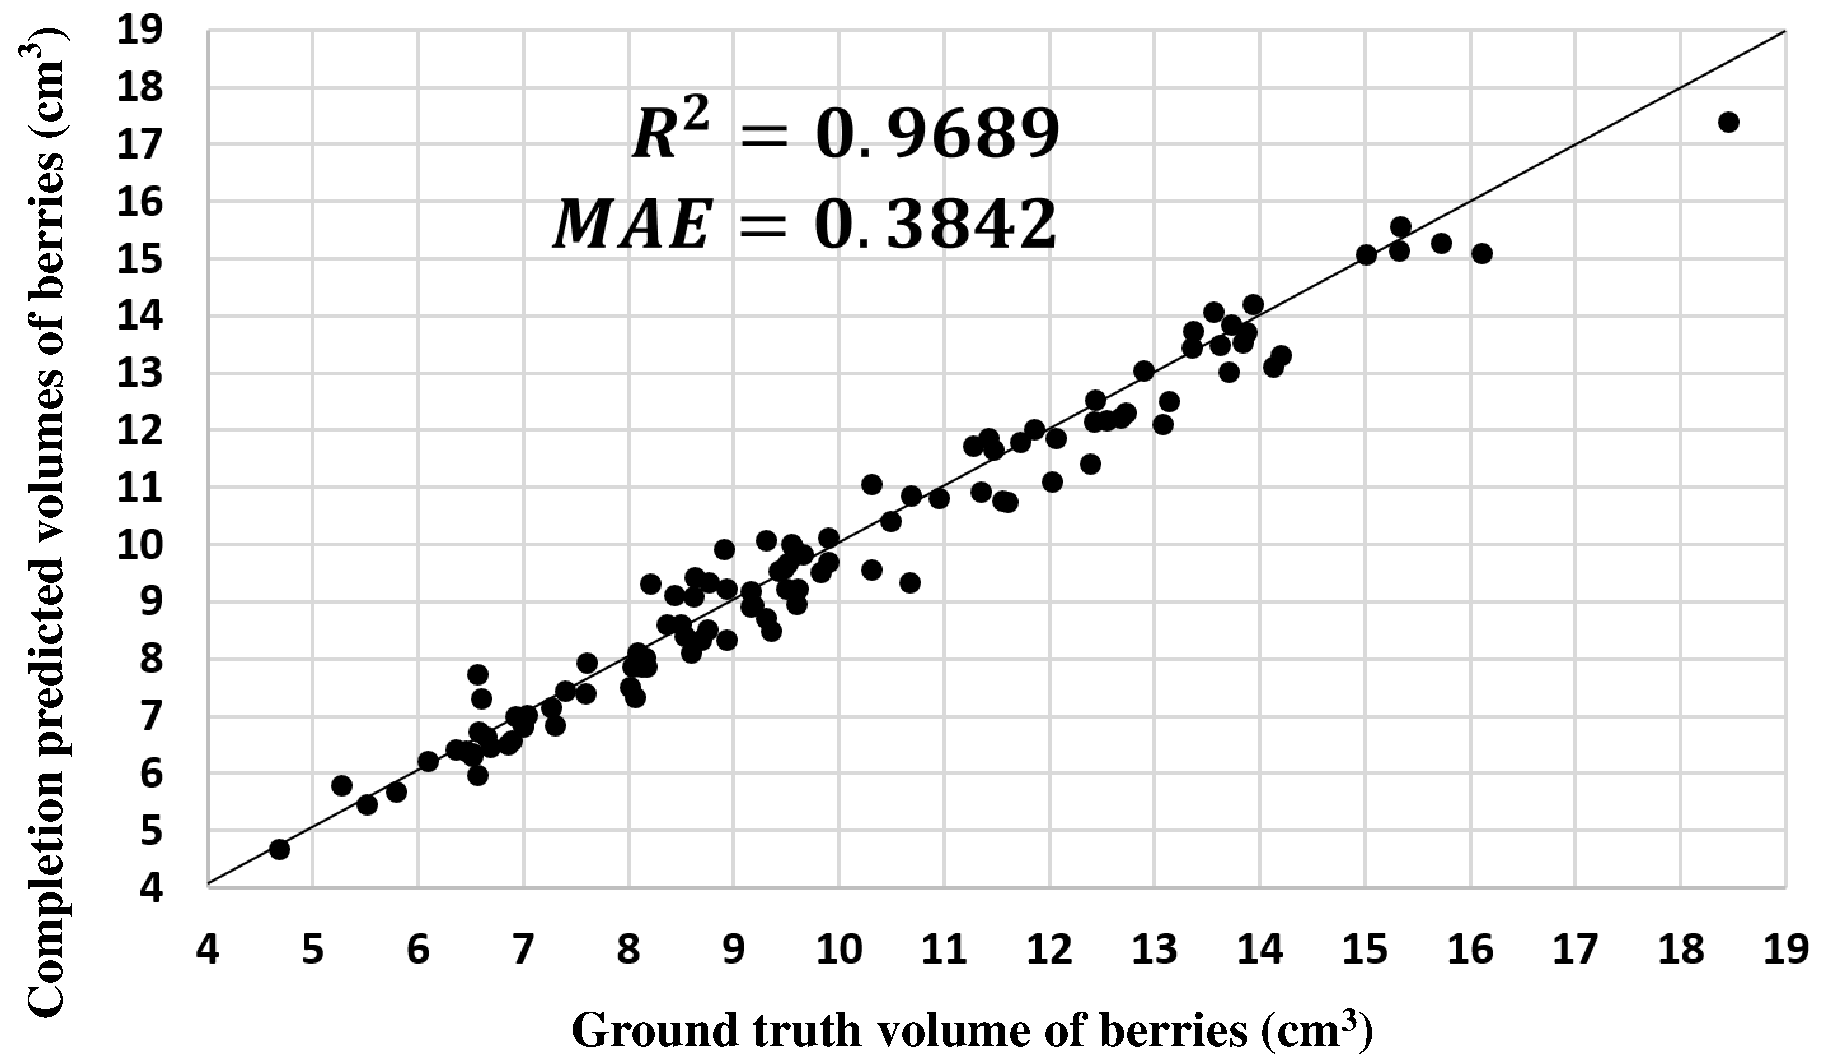
\includegraphics[width=1\textwidth]{figures/Figure15.pdf}
    \caption{Experimental results of berry volume calculation. \added{The ground truth values are obtained by completely scanning berries that were separated from the bunch (Fig.~\ref{fig:raw9}b1); The predicted values are obtained from our proposed self-supervised completion method, which addresses incomplete scans of berries that occur due to occlusion while they were still attached to the bunch (Fig.~\ref{fig:raw9}a2).}}
    \label{fig:raw18}
\end{figure}

The experimental results showed that the proposed method achieved \added{both} high accuracy in the calculation of the radius \added{and volumes} of different grape species.
\added{In out study, we achieved an average $R^2$ of 0.86 and an average MAE of 0.608 mm across the three axis of berry, as well as an $R^2$ of 0.9689 and an MAE of 0.3842 $cm^3$ for berry volumes.}
\added{By comparision, \citet[Fig.~4]{rist_highprecision_2018} reported $R^2$ values of 0.54, 0.85, and 0.83 for berry width, length, and volume, respectively.}
\added{\citet{botturi_stewie_2023} reported a best-case MAE of 21.7mm for berry ratio estimataion using deep learning network on 2D images.}
\added{Although the method by \citet{ni_threedimensional_2021} achieved a lower errors for volume estimataion (RMSE of 0.292 $cm^3$), it relies on sphere fitting that are primarily applicable to clustered, round fruits.}
\added{In contrast, our proposed method not only accounts for occluded areas but is also adaptable to fruits of varying shapes, if appropriate paired training data is available.}

\section{Discussion}

% achievement and contribution of ths study
In this paper, \replaced{an automated deep learning pipeline for}{a method for the automatic} acquisition of 3D phenotypic traits of grape \added{bunch} was presented to address the problems of high labor cost, poor accuracy, and inability to realize end-to-end analysis. 
\replaced{As a major contribution}{Moreover}, to address the problem of incomplete point clouds of berries due to occlusion, we introduced GrapeCPNet, a berry point cloud completion model based on the self-supervised training method.
\deleted{Based on the point cloud of a grape bunch, a combination of deep learning point cloud processing algorithms realized the counting of the number of berries, the calculation of berry radius, and berry volume. }

% revisiting background to reboot reader
\added{Grape berry counting and size estimation plays a critical role in vineyard management and yield prediction.}
\added{By using common digital cameras alongside deep learning networks, several studies have achieved automatic berry detection and instance segmentation \citep{jadhav_comparative_2021, chen_instance_2023}, and then forward the analyses of geometry traits and yield estimation \citep{quinones_gcnet_2025}.}
\added{However, because of the dense and compact arrangement of berries within a grape bunch, some portions are often occluded and not visible when relying solely on single 2D images.}
\added{To reduce the effects of occlusion, \citet{du_instance_2023} reported accurate berry counting estimations by correlating image-based detections with ground measurements.}
\added{However, applying this method to other vineyards requires extensive, labor-intensive ground measurements}
\added{Similarly, \citet{botturi_stewie_2023} attempted to extract feature maps, such as berry radii, directly from deep networks applied to 2D images}
\added{Despite this approach, it still suffers from information loss and resulted in a high MAE of 21.7 mm.}
\added{Applying multi-view images for 3D reconstruction can significantly reduce the extent of occlusion caused by viewpoint limitations.}
\added{But unlike 2D images, which have well-structured data in the form of organized pixel matrices, the unordered nature of points in a 3D point cloud introduces significant challenges.}
\added{Meanwhile, the inner portion of berry is still invisible, only the surface of exposed berry surfaces can be scanned or reconstructed.}
\added{This complicates the algorithm design for individual berry segmentation and accurate berry size estimation.}

% revisit gap/aim/method
\added{For individual berry segmentation, early studies relied on the circular characteristics of the visible portions of berries for segmentation.}
\added{Building on the work of \citet{schnabel_efficient_2007}, who introduced point cloud shape detection using RANSAC, researchers were able to cluster partial berries based on their rounded shapes \citep{scholer_automated_2015, rist_highprecision_2018, schneider_predicting_2020}.}
\added{However, this feature-based approach performs well only in sparse grape arrangements and proves ineffective in more complex, dense conditions.}
\added{The reliance on manually designed features for algorithm development has now reached its limitations.}
\added{With advancements in machine learning, the focus has shifted to a data-driven era, where algorithms can learn complex feature patterns automatically.}
\added{For instance, \citet{rose_automated_2016} applied machine learning to distinguish features between grape berry clusters and background leaves automatically.}
\added{Similarly, \citet{ni_threedimensional_2021} implemented a two-step approach by first using mature 2D instance segmentation techniques on 2D images and then projecting the resulting segmentation masks onto reconstructed 3D models to complete the challenging task of 3D instance segmentation.}
\added{In another approach, \citet{luo_3d_2023} Mask R-CNN for 2D image segmentation and projected the results onto RGB-D point clouds.}
\added{The normal directions derived from the point clouds were then packed as an additional feature in the PointNet++ network for point cloud segmentation.}
\added{In this study, we applied the state-of-the-art point cloud segmentation network, SoftGroup \citep{vu_softgroup_2022} directly to the problem.}
\added{The primary time-consuming work of our approach was the annotation of 3D data for instance segmentation.}
\added{Compared to similar studies on grape berries, our proposed method demonstrated superior performance, achieving the best results among the reviewed methods (Subsection~\ref{sec:insegresults}).}

\added{For berry completion using deep learning, the most challenging and time-consuming task is preparing the paired training datasets of complete and incomplete point clouds.}
\added{In our previous work on potato tuber completion networks \citep{blok_highthroughput_2025}, a distinguishable pin was used as a reference point to align the complete tuber scans obtained via photogrammetry with the incomplete tuber scans captured using an RGB-D camera.}
\added{A pin-guided point cloud matching algorithm was then applied to calculate the transformation matrix for pairing the datasets.}
\added{Potato tubers, being single objects with clear textures and shape variation, presented fewer challenges when aligning data collected by two different types of sensors.}
\added{However, grape berries pose a significantly more difficult problem due to their highly rounded shapes, weak texture features, and strong reflectance, which complicates the creation of paired data.}
\added{As a result, the previous pin-guided point cloud pairing method used for potato tuber datasets is not effective for grape berries.}
\added{Thus, we simulated random sphere cutting on the complete berry point clouds to generate thousands of paired incomplete point clouds, as described in Subsection~\ref{sec:berrycut}.}
\added{As demonstrated in Subsection~\ref{sec:32}, these automatically generated paired training datasets were successfully used to train several completion models (Table~\ref{tbl:4}).}
We have found that some researchers \citep{pan_panoptic_2023,magistri_efficient_2024} have improved the completion effect by encoding a prior knowledge of the geometry of the object into the weights of the neural network. 
\added{Considering the agricultural plant completion task, our proposed GrapeCPNet, which combines centroid-based sparse completion with diffusion-based dense completion, outperformed other networks in terms of performance.}
We found that GrapeCPNet \replaced{performed a little bit worse}{effective} in the case of \replaced{strange}{complex} berry \replaced{shapes}{appearance}, such as drop-shaped.
We subsequently consider utilizing the prior knowledge of berry geometry to achieve more detailed morphological feature extraction and representation to improve the quality of completion. 

% challenges, limitations and future works.
\added{Another limitation of this study is that it focused on a single berry bunch in a controlled environment.}
The noise in the data is also related to the effectiveness of the method proposed in this paper.
\added{For practical applications in vineyards, collecting the same point cloud quality as that achieved in controlled indoor environments can be challenging, and multi-view data collection may not be as efficient.}
How to \added{effectively} implement the method in practical application scenarios\deleted{, such as RGB-D collected point cloud data,} is another issue to be considered in future research.
\added{To increasing data collection efficiency, devices such as RGB-D cameras \citep{blok_highthroughput_2025}, fisheye cameras \citep{tamura_unsupervised_2025}, or even 360 cameras can be used.}
\added{Moreover, as in previous studies \citep{rose_automated_2016, luo_3d_2023}, investigating methods to segment individual grape bunches directly from vineyard scans using deep learning techniques should be an area of future exploration.}
\added{Additionally, \citet[Fig.~9]{scholer_automated_2015} successfully demonstrated the construction of virtual 3D models of grape bunches, including the hidden branching architecture. }
\added{By collecting time-series growth data, the branching structure could potentially be captured during early stages of thinning, as suggested by \citep{du_instance_2023}.}
\added{Such data could enable studies on growth prediction for optimizing harvesting times and assessments of branching structure deviations within crowded berry bunches.}
\added{Finally, applying the latest procedural computer graphics (CG) modeling techniques \citep{karoly_automated_2022} or functional-structural plant models \citep{helmrich_scalable_2024} represents another promising approach to advancing practical applications in this field.}

% the achievement / impact of study / potential applications.
Through the method proposed in this paper, the automated acquisition of 3D phenotypic traits of grape can be realized, which is of great significance in the field of agricultural production and scientific research. 
First, there are large differences in berry morphology among different species of grape, and accurate reconstruction and analysis at the berry-level can help researchers analyze character differences more accurately. 
This plays an important role in plant breeding, cultivation management, and yield prediction. 
Secondly, the point cloud data analysis technology based on 3D reconstruction has a wide application of field crop analysis. 
Through the designed data acquisition method and related technologies, combined with the actual field crop growing environment, the growth process can be monitored and analyzed in real-time. 
Further, it can help understanding the phenotypic change of crops in natural growing environments, providing better and objective measures for crop production and quality control. 

\section{Conclusion}

\added{In this study, we proposed a deep-learning-based pipeline for processing 3D phenotyping grape bunches reconstructed by photogrammetry.}
\added{The major contribution is the self-supervised completion network, named GrapeCPNet, designed to address the problem of missing parts in berries occluded within grape bunches with few manual annotations.}
\added{We utilized state-of-the-art, data-driven deep learning approaches to address these challenges.}
\added{First, the SoftGroup network, utilizing segmentation annotations from 8 grape bunches, was used to train a data-driven berry instance segmentation model.}
% \added{By randomly producing missing areas from complete berries, we automatically generated large number of training data for completion tasks.}
\added{The proposed GrapeCPNet also achieved better performance than existing completion networks, with Precision of 0.729, Recall of 0.772 and F-score of 0.751.}
\added{The ellipsoid surface fitting, used to calculate three axis lengths and volumes, achieved an average $R^2$ of 0.86 and 0.97 respectively, when comparing completed berries with their ground truth.}
\added{This study clearly demonstrates the potential of using data-drive strategies with minimal annotation effort to address the 3D occlsuion challenge in agricultural applications.}
\added{Although this network has only been tested on grape bunches collected in a controlled indoor environment, the proposed deep learning pipelines and training data generation approach have broad potential applications for in-field vineyards and even other crops in the future.}

\section*{CRediT authorship contribution statement}
\textbf{Wenli Zhang}: conceptualization, methodology, supervision, funding acquisition, project administration, writing - review; \textbf{Chao Zheng}: methodology, software, data curation, writing - original draft \& editing; \textbf{Chenhuizi Wang}: data curation, software; \textbf{Pieter M. Blok}: methodology, supervision, writing - review \& editing; \textbf{Haozhou Wang}: methodology, writing - review \& editing; \textbf{Wei Guo}: conceptualization, methodology, funding acquisition, supervision, writing - review \& editing.

\section*{Declaration of generative AI and AI-assisted technologies in the writing process.}
During the preparation of this work the authors used ChatGPT in order to check grammar, spelling, and improve fluency. After using this tool/service, the authors reviewed and edited the content as needed and take full responsibility for the content of the published article.

\section*{Declaration of competing interest}
The authors declare that they have no known competing financial interests or personal relationships that could have appeared to influence the work reported in this paper.

\section*{Data availability}
The dataset and model weight for the test usage is available here: https://github.com/I3-Laboratory/GrapeCPNet. The whole dataset used in this paper is available upon request.

\section*{Funding}
This study was partially supported by the National Natural Science Foundation of China (NSFC) Program 62276009 and the Japan Science and Technology Agency (JST) AIP Acceleration Research JPMJCR21U3, the Hokkaido Sarabetsu Village “Endowed Chair for Field Phenomics” project.

% \section*{Acknowledgements}
% We would like to thank ...

{\clearpage}

\bibliographystyle{elsarticle-harv}
\setcitestyle{aysep={}}
\bibliography{references}

\end{document}
